\documentclass[11pt]{report}
\usepackage[margin=1.1in]{geometry}
\usepackage[utf8]{inputenc}
\usepackage[italian]{babel}
\usepackage{amssymb} 
\usepackage{amsmath}
\usepackage{amsthm}
\usepackage{thmtools}
\usepackage{multicol}
%\usepackage{marginnote}
\usepackage{url}
\usepackage{pdfpages}
\usepackage{hyperref}
\usepackage{centernot}
\usepackage{marginnote}

\setcounter{tocdepth}{3}
\setcounter{secnumdepth}{3}

\usepackage{subcaption}

\begin{document}
\renewcommand{\contentsname}{Indice degli appunti}
\title{\textbf{Progettazione web - A.A.2020-2021}}
\author{Gabriele Frassi}
\maketitle

\small\tableofcontents\normalsize

\part{Lezioni di Marcelloni}
\chapter{Introduzione}
\section*{Argomenti del corso}
Nel corso di progettazione web cercheremo di capire come sviluppare un'applicazione web. Ci occuperemo principalmente di sviluppare applicazioni web seguendo gli standard: questo permetterà di ridurre problemi di compatibilità nel passaggio da un browser a un altro. Il corso riguarderà le seguenti tecnologie
\begin{itemize}
\item HTML 5.0, linguaggio ipertestuale per descrivere contenuti fruibili via web
\item CSS, cascade style sheets, per quanto riguarda l'aspetto estetico
\item Client-side: Javascript
\item Server-side: PHP
\end{itemize}
Svilupperemo siti sfruttando tutte queste tecnologie (occupandoci sia della client-side che della server-side). Oltre a questo studieremo il protocollo HTTP. Si consiglia caldamente di seguire i laboratori.

\section*{Cos'è il \emph{World Wide Web}?}
Con World Wide Web intendiamo una rete di risorse e informazioni di vario tipo. Fino a dieci anni fa i siti erano composti sostanzialmente da testo (documenti hypertext): adesso le cose sono decisamente più complesse. Adesso, con documenti multimediali come immagini, audio e video, parliamo di documenti hypermedia. Tutto questo può essere visto attraverso i browser, che interpretano dei linguaggi ipertestuali. 

\paragraph{Rispetto dei linguaggi} Se rispettiamo gli standard dei linguaggi l'interprete garantisce una grande portabilità, e la quasi certezza che i browser principali interpretino correttamente quanto scritto da noi.

\paragraph{Protocollo client-server} I contenuti sono presenti su server remoti, e sono accessibili grazie al protocollo client-server http (un protocollo richiesta-risposta): il client richiede la risorsa, e il server la restituisce. Il protocollo è \emph{stateless}: il server non riconosce il client e non salva le sue richieste. Questo significa che in caso di perdita di connessione non sarà possibile recuperare quanto fatto prima (quindi la richiesta dovrà essere ripetuta).

\section*{Struttura di progetto}
Il nostro progetto si strutturerà in tre livelli:
\begin{itemize}
\item \textbf{Contenuto}: con HTML formattiamo il testo: stabiliamo cosa sia il titolo di un articolo, quali sono le sezioni dell'articolo. Indichiamo ciò che vogliamo rendere accessibile ai visitatori.
\item \textbf{Presentazione}: con CSS stabiliamo quale sarà l'aspetto del nostro contenuto. La cosa è molto sentita oggi, soprattutto in un mondo con dispositivi aventi dimensioni di schermo diverse. Dobbiamo prevedere diversi stili di presentazione in modo tale che il sito sia fruibili su tutti i dispositivi. Col CSS possiamo stabilire, in aggiunta, come stampare un documento (cosa mostrare e non mostrare nella stampa). Non è obbligatorio definire tutti gli aspetti grafici: i browser presentano dei modelli di presentazione default.
\item \textbf{Comportamento}: con Javascript implementeremo applicazioni che interagiscono dinamicamente con l'utente. Possiamo porre, per esempio, dei bottoni: noi non solo poniamo il bottone, ma dobbiamo indicare anche cosa farà quel bottone. Possiamo richiedere, per esempio, che i campi compilati da un utente siano stati inseriti in modo corretto. Altro scopo importante del Javascript è la possibilità di compiere verifiche lato client sul contenuto posto dall'utente (verificare che un CAP esista, che il cognome consiste in una sequenza formata solo da caratteri, tutti i controlli che non necessitano di informazioni variabili nel tempo)
\end{itemize}
\paragraph{E il PHP?} Questo linguaggio viene utilizzato per generare contenuti HTML-CSS (lato client) o per interagire con basi di dati (lato server). Il PHP ha peso minore rispetto agli altri tre linguaggi: o produce il livello contesto o il livello presentazione.
\paragraph{Controlli lato server} Altre cose, come per esempio la verifica della presenza di eventuali duplicati (per esempio l'username al momento della registrazione) necessitano di un controllo lato server (devo per forza connettermi al database).
\paragraph{Controlli tutti in lato server?} Non si potrebbe fare ogni controllo in PHP e risparmiarsi il javascript? La cosa è sconsigliata: con javascript possiamo dire in modo immediato all'utente che qualcosa non va ed evitare traffico di rete inutile.

\section*{Pilastri su cui si fonda il WWW}
Il World Wide Web si poggia su tre meccanismi base:
\begin{itemize}
\item Assegnazione di nomi in modo uniforme (devo poter identificare una risorsa in modo univoco)
\item Protocolli, le regole per accedere ai contenuti
\item Ipertesti (Hypertext), collegamenti ad altri documenti posti nella nostra pagina. La cosa è grandiosa e permette di passare da una pagina a un'altra del nostro sito.
\end{itemize}
\subsection*{URI (\emph{Uniform resource indicator})}
Ogni informazione presente sul web presenta un indirizzo, codificabile attraverso un URI (Uniform Resource Identifier): con esso intendiamo
\begin{verbatim}<scheme>:<scheme-specific-part>\end{verbatim}
\begin{itemize}
\item con scheme intendiamo il nome del meccanismo utilizzato per accedere alle risorse (http, per esempio)
\item con scheme-specific-part intendiamo il nome della macchina che ospita la nostra risorsa e l'eventuale percorso per raggiungere la risorsa stessa
\end{itemize}
L'URI può essere un indirizzo (e a quel punto si parla di URL, \emph{Uniform resource Locator}) o un nome (UNR, \emph{Uniform resource name}). In un certo senso possiamo dire che:
\begin{itemize}
\item con URN abbiamo il nome della persona. Un esempio è il seguente
\begin{verbatim}
urn:isbn:0-395-36341-1
\end{verbatim}
\item con URL abbiamo l'indirizzo di una persona. Un esempio è il seguente
\begin{verbatim}
http://www.w3.org/TR
\end{verbatim}
\end{itemize}
\paragraph{Fragmente identifier} Con l'URI possiamo fare riferimento a un'area precisa del nostro documento (quando poniamo il cancelletto)
\begin{verbatim}
http://www.w3.org/TR#nome_id
\end{verbatim}
\paragraph{Relative URI} In alcuni casi andiamo a porre l'URI senza indicare lo \emph{scheme}. Un esempio è nel codice HTML quando poniamo un immagine: poniamo semplicemente il \emph{path}, senza indicare il dominio dove è presente la risorsa.

\subsection*{Protocolli}
I protocolli principali sono i seguenti:
\begin{itemize}
\item http, \emph{Hypertext transfer protocol} (oggi è presente anche l'https, che garantisce maggiore sicurezza impedendo - teoricamente - il furto di dati da parte di malintenzionati)
\item ftp, \emph{File transfer protocol}. Protocollo per il trasferimento di file
\item mailto (\emph{electronic mail address}), per gestire indirizzi mail.
\item file (caricamento di file specifici sul browser)
\end{itemize}
Ricordare quanto detto all'inizio relativamente al protocollo HTTP.

\chapter{HTML}

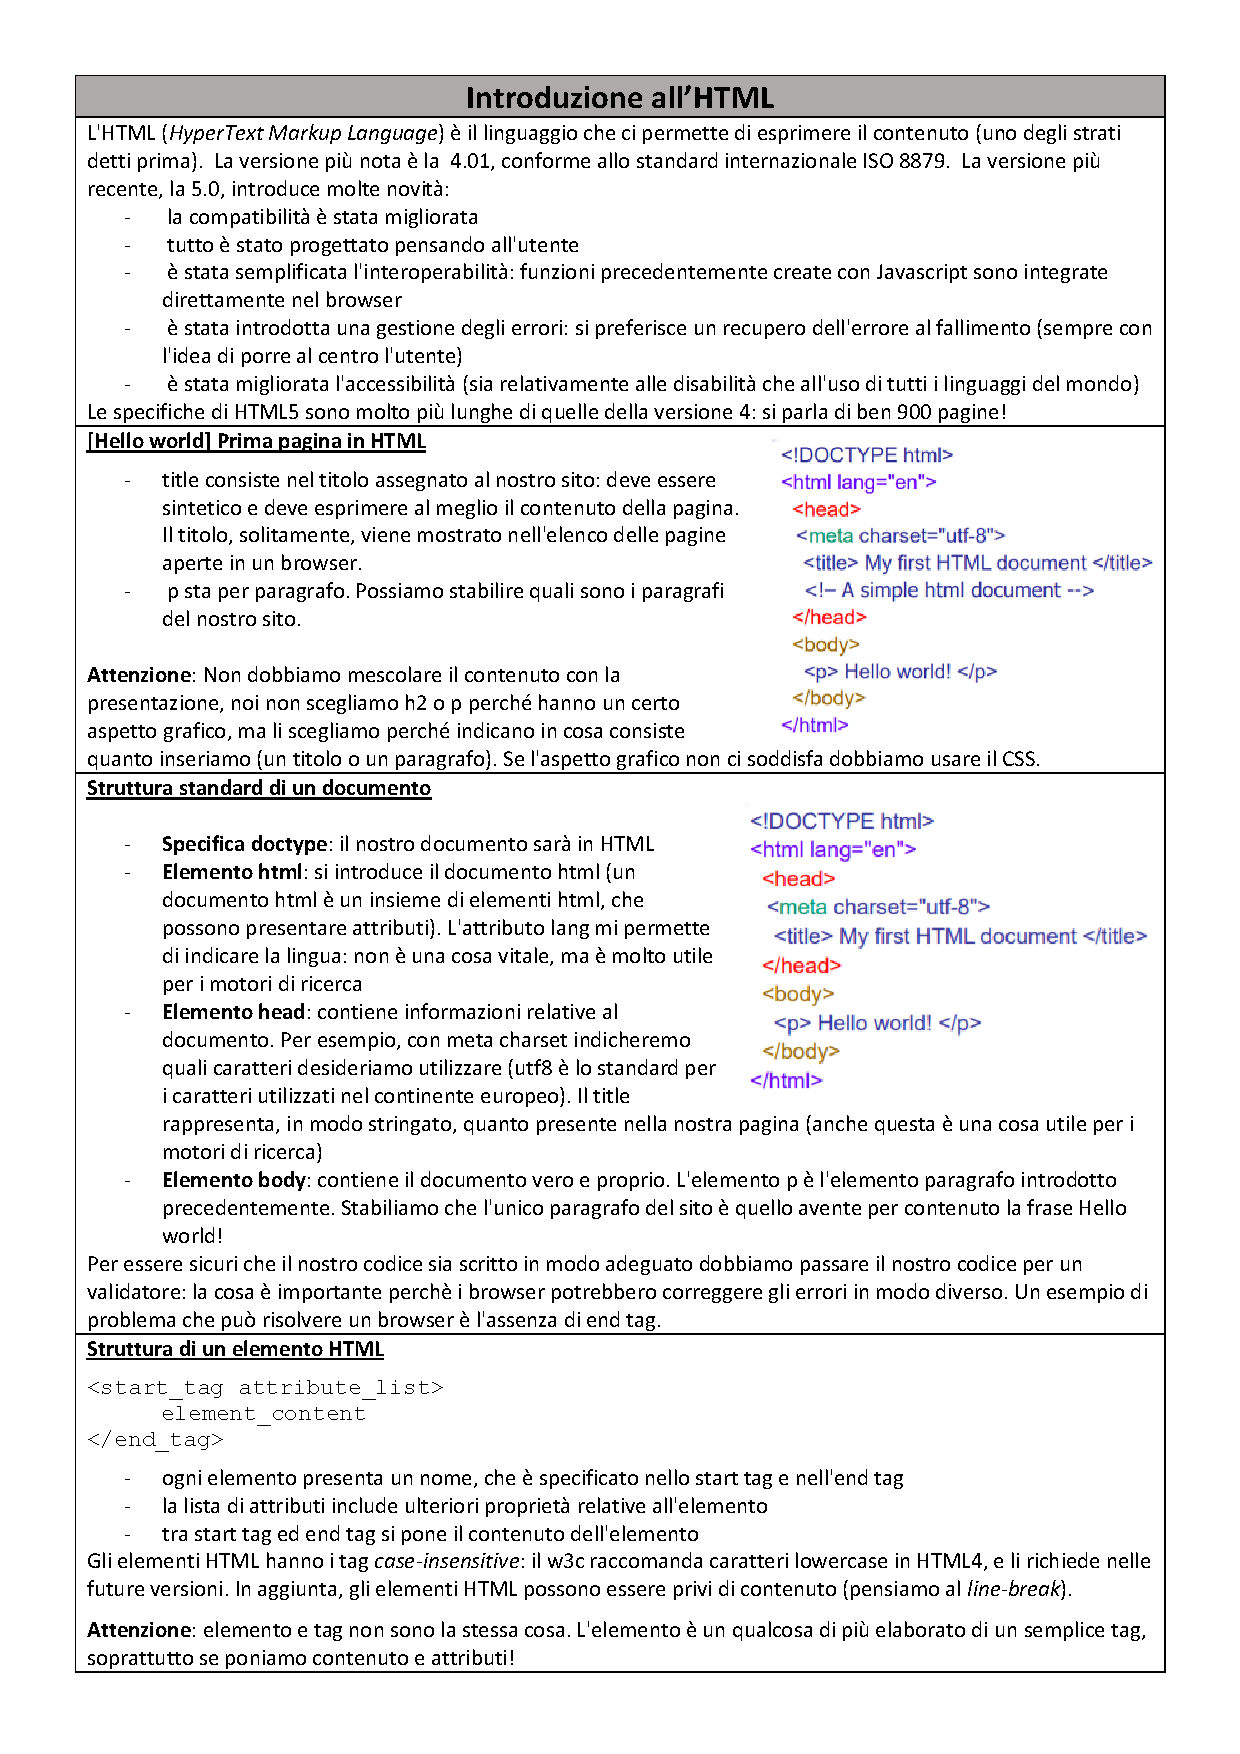
\includepdf[pagecommand={\thispagestyle{plain}},scale=0.92,pages=-]{pdf/html}

\chapter{CSS}
Oggi vedremo il CSS (Cascading Style Sheets): esso consiste nel linguaggio che ci permette di definire uno stile di presentazione per il contenuto formattato. 
\paragraph{Separazione contenuto e presentazione} La separazione tra contenuto e presentazione permette, come già detto, di impostare più stili per uno stesso contenuto. La cosa è vantaggiosa anche dal punto di vista della banda: la memorizzazione del foglio di stile nella cache permette di caricare con maggiore efficienza siti già visitati precedentemente. Altro dettaglio è la semplificazione nelle modifiche: meglio modificare un solo file che 1000 file per le stesse cose!

\paragraph{Attuale specifica} La versione attuale del CSS è la CSS3: essa è intervenuta moderando le aspirazioni della specifica CSS2 (molte cose erano difficili da implementare nei browser).

\section*{Come inseriamo codice CSS nel documento HTML?}
\subsection*{Inline styles}
\begin{center}

\includegraphics{img/2.PNG}
\end{center}
Possiamo inserire le regole di CSS all'interno dell'attributo style relativo a un certo elemento HTML. L'uso di questo metodo deve essere moderato il più possibile: si riduce al minimo la distinzione tra contenuto e presentazione.
\subsection*{Internal Style Sheet}
La seconda possibile è porre un elemento style all'interno dell'head. Con l'attributo type specifichiamo che quanto stiamo inserendo sono regole di css (text/css), con l'attributo media indichiamo dove sono valide le nostre regole. 
\begin{center}
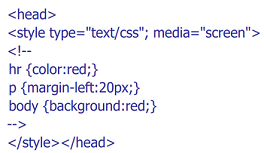
\includegraphics{img/3.PNG}
\end{center}
\paragraph{Metodica vecchia} Era abitudine (adesso non più) di porre il contenuto dello style come un commento. La cosa era necessaria: i browser, molti anni fa, potevano non interpretare codice CSS (in caso di fallimento nell'interpretazione del CSS il porlo come commento permetteva di nasconderlo nell'output).

\subsection*{External Style Sheet}
L'ultima possibilità, la migliore, consiste nel porre le regole di CSS in un file a parte. Questo sarà riferito nel documento principale attraverso un elemento link o una @import rule in un elemento style.
\paragraph{Elemento link} Il primo metodo è utilizzare l'elemento link con gli attributi rel, type ed href. Il tag sarà posto nell'head
\begin{center}
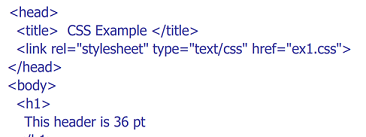
\includegraphics{img/4.PNG}
\end{center}
\paragraph{Direttiva import} Il secondo metodo è il ricorso alla direttiva import, posta all'interno dell'elemento style. Stabiliamo che vogliamo importare il contenuto di un file CSS
\begin{center}
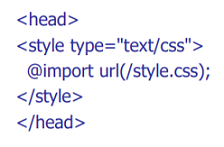
\includegraphics{img/5.PNG}
\end{center}
\paragraph{Media type} Abbiamo già affermato che è possibile porre style sheets diversi in base al media, cioè al dispositivo utilizzato. Possiamo porre uno stile grafico per chi visualizza il sito da schermo, ma anche porre uno stile grafico valido solo al momento della stampa. Alla diapositiva 20 del CSS è presente una lista di media.
\paragraph{import at-rule e media-at-rules} Nella direttiva import possiamo stabilire anche il media. Possiamo anche stabilire, all'interno di CSS in un elemento style, le situazioni a cui si applicherà una parte del codice CSS (media-at-rules).
\begin{center}
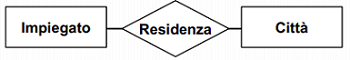
\includegraphics{img/6.PNG}
\end{center}

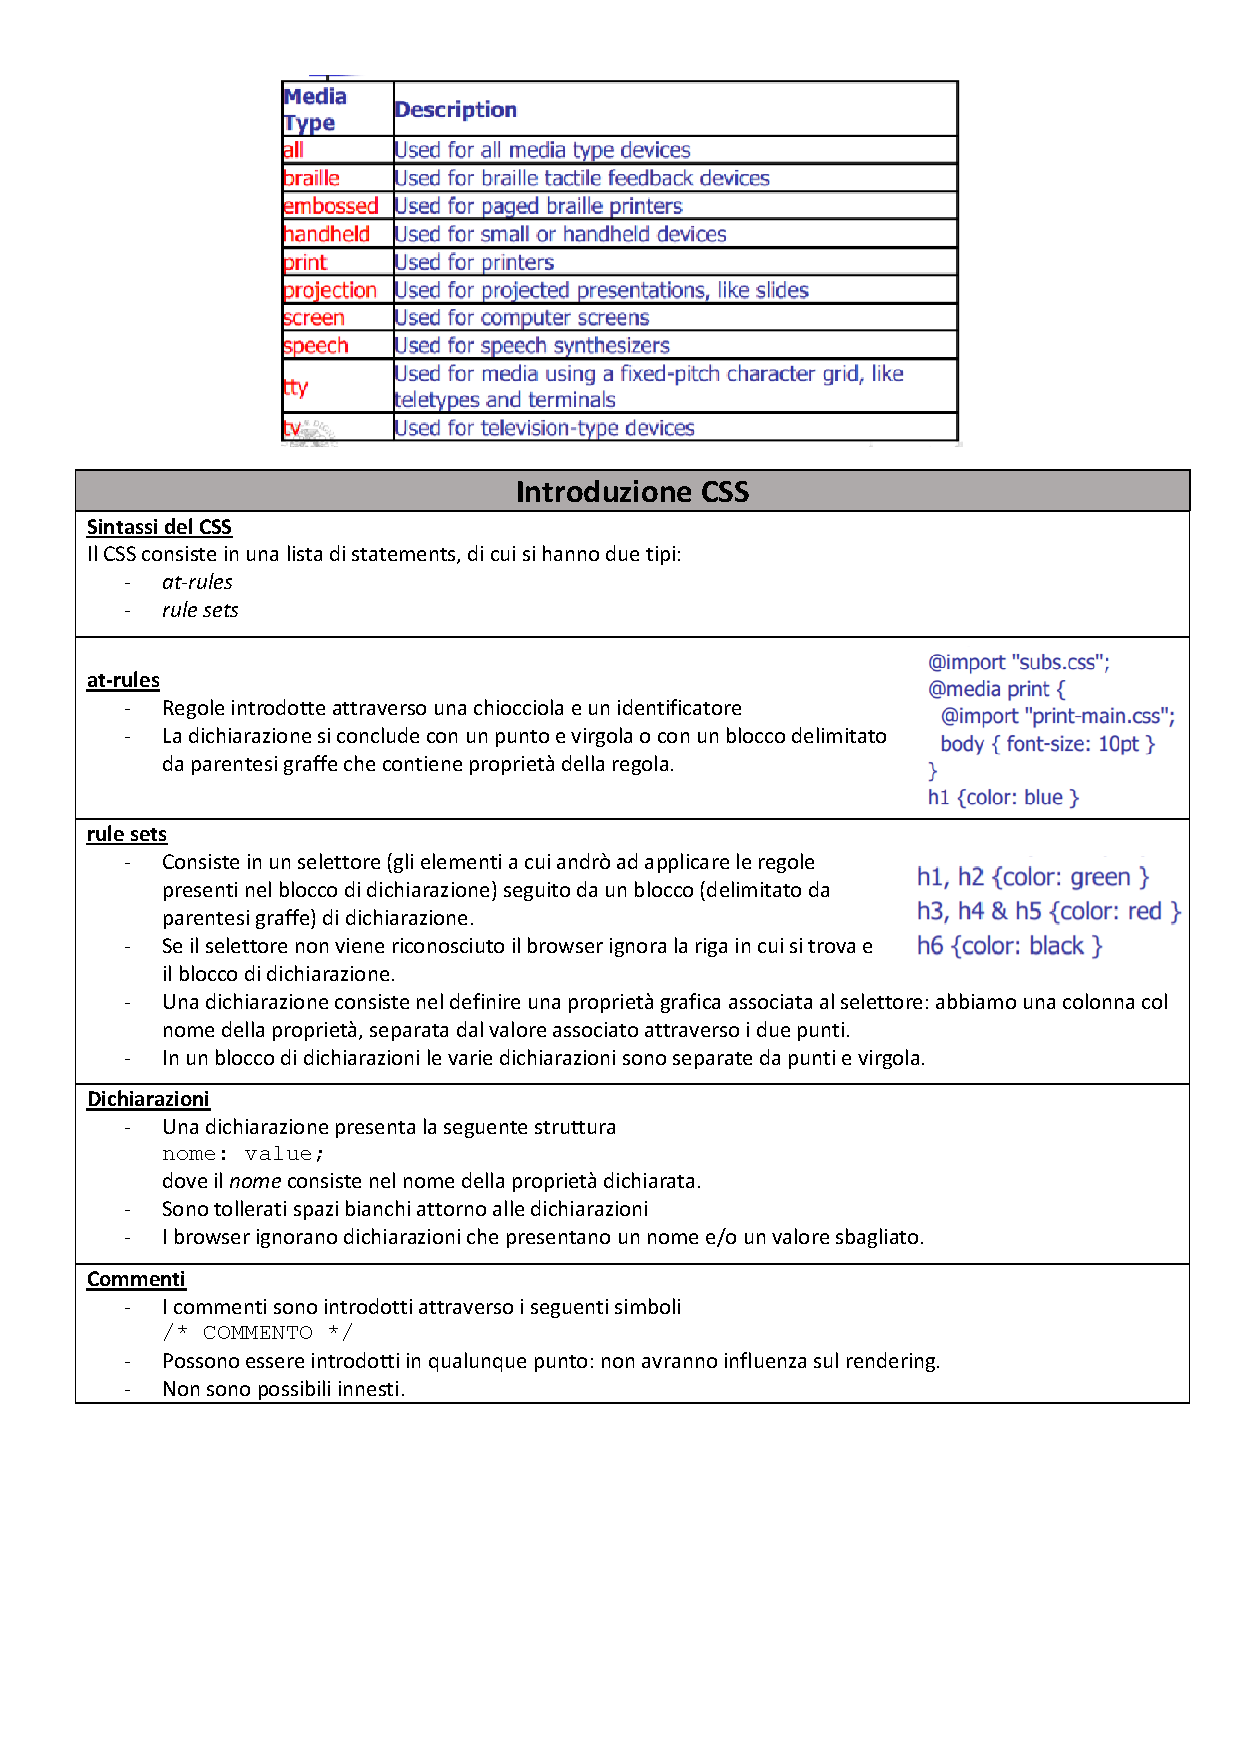
\includepdf[pagecommand={\thispagestyle{plain}},scale=0.92,pages=-]{pdf/css1}
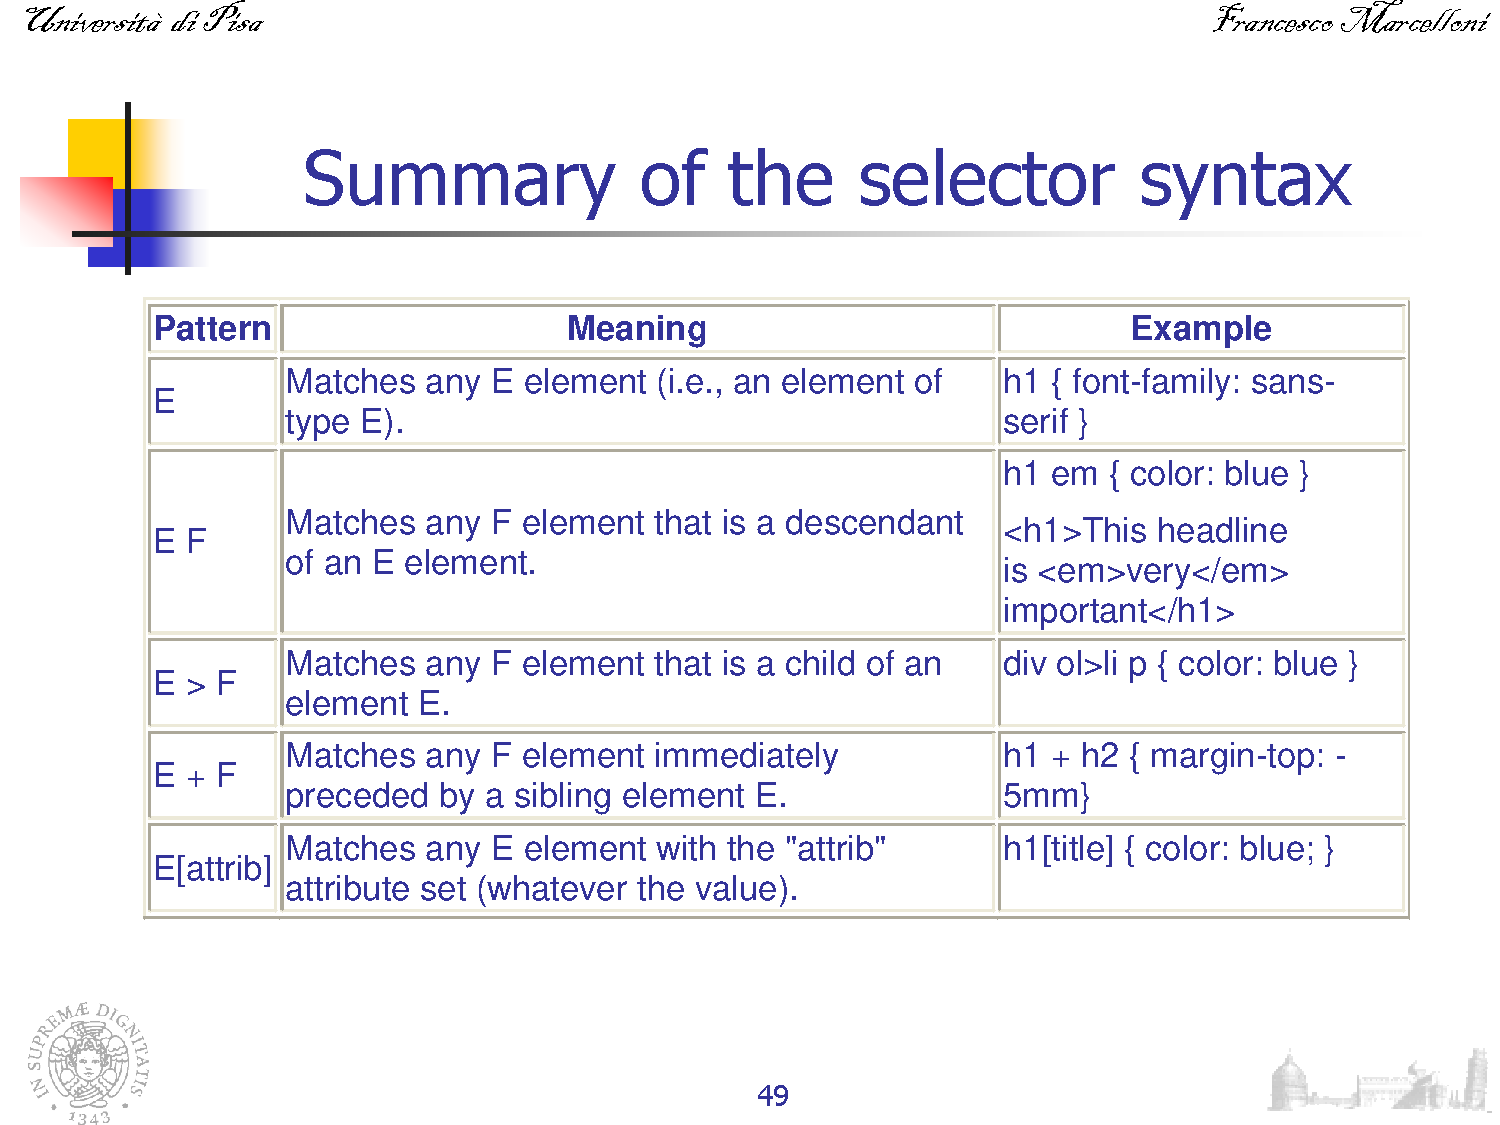
\includepdf[pagecommand={\thispagestyle{empty}},scale=0.95,frame, nup=2x3, pages=-]{pdf/sintassiselettori1}
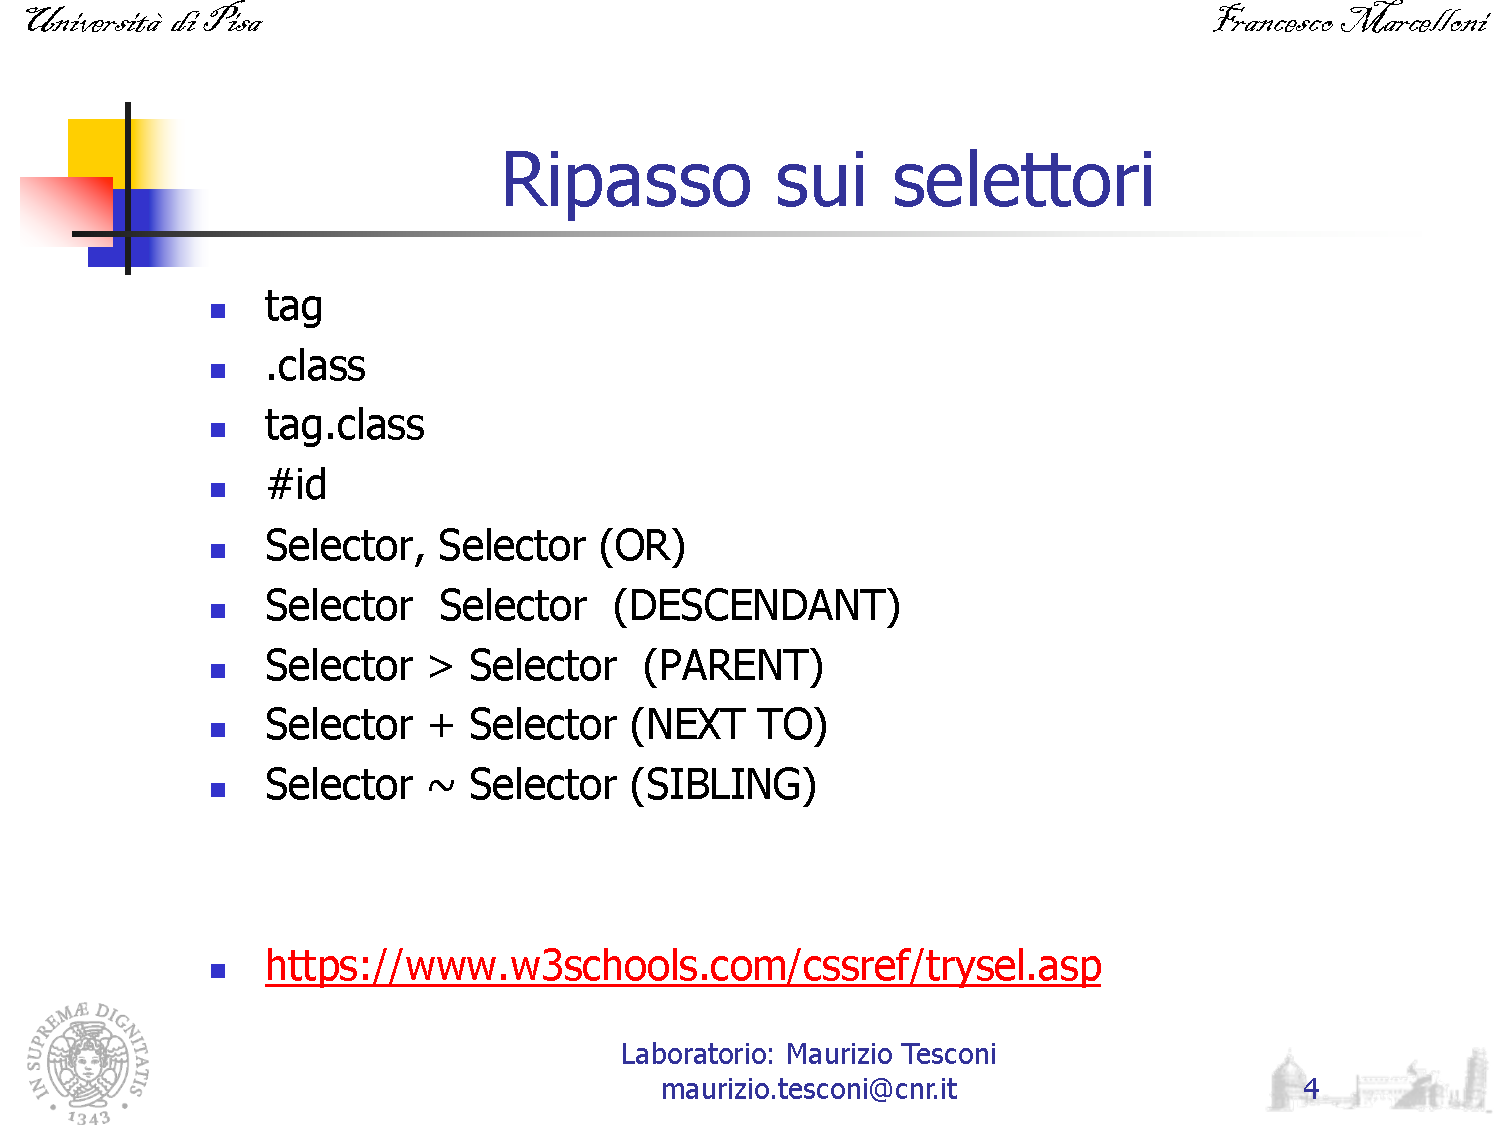
\includepdf[pagecommand={\thispagestyle{empty}},scale=0.95,frame, nup=2x3, pages=-]{pdf/sintassiselettori2}
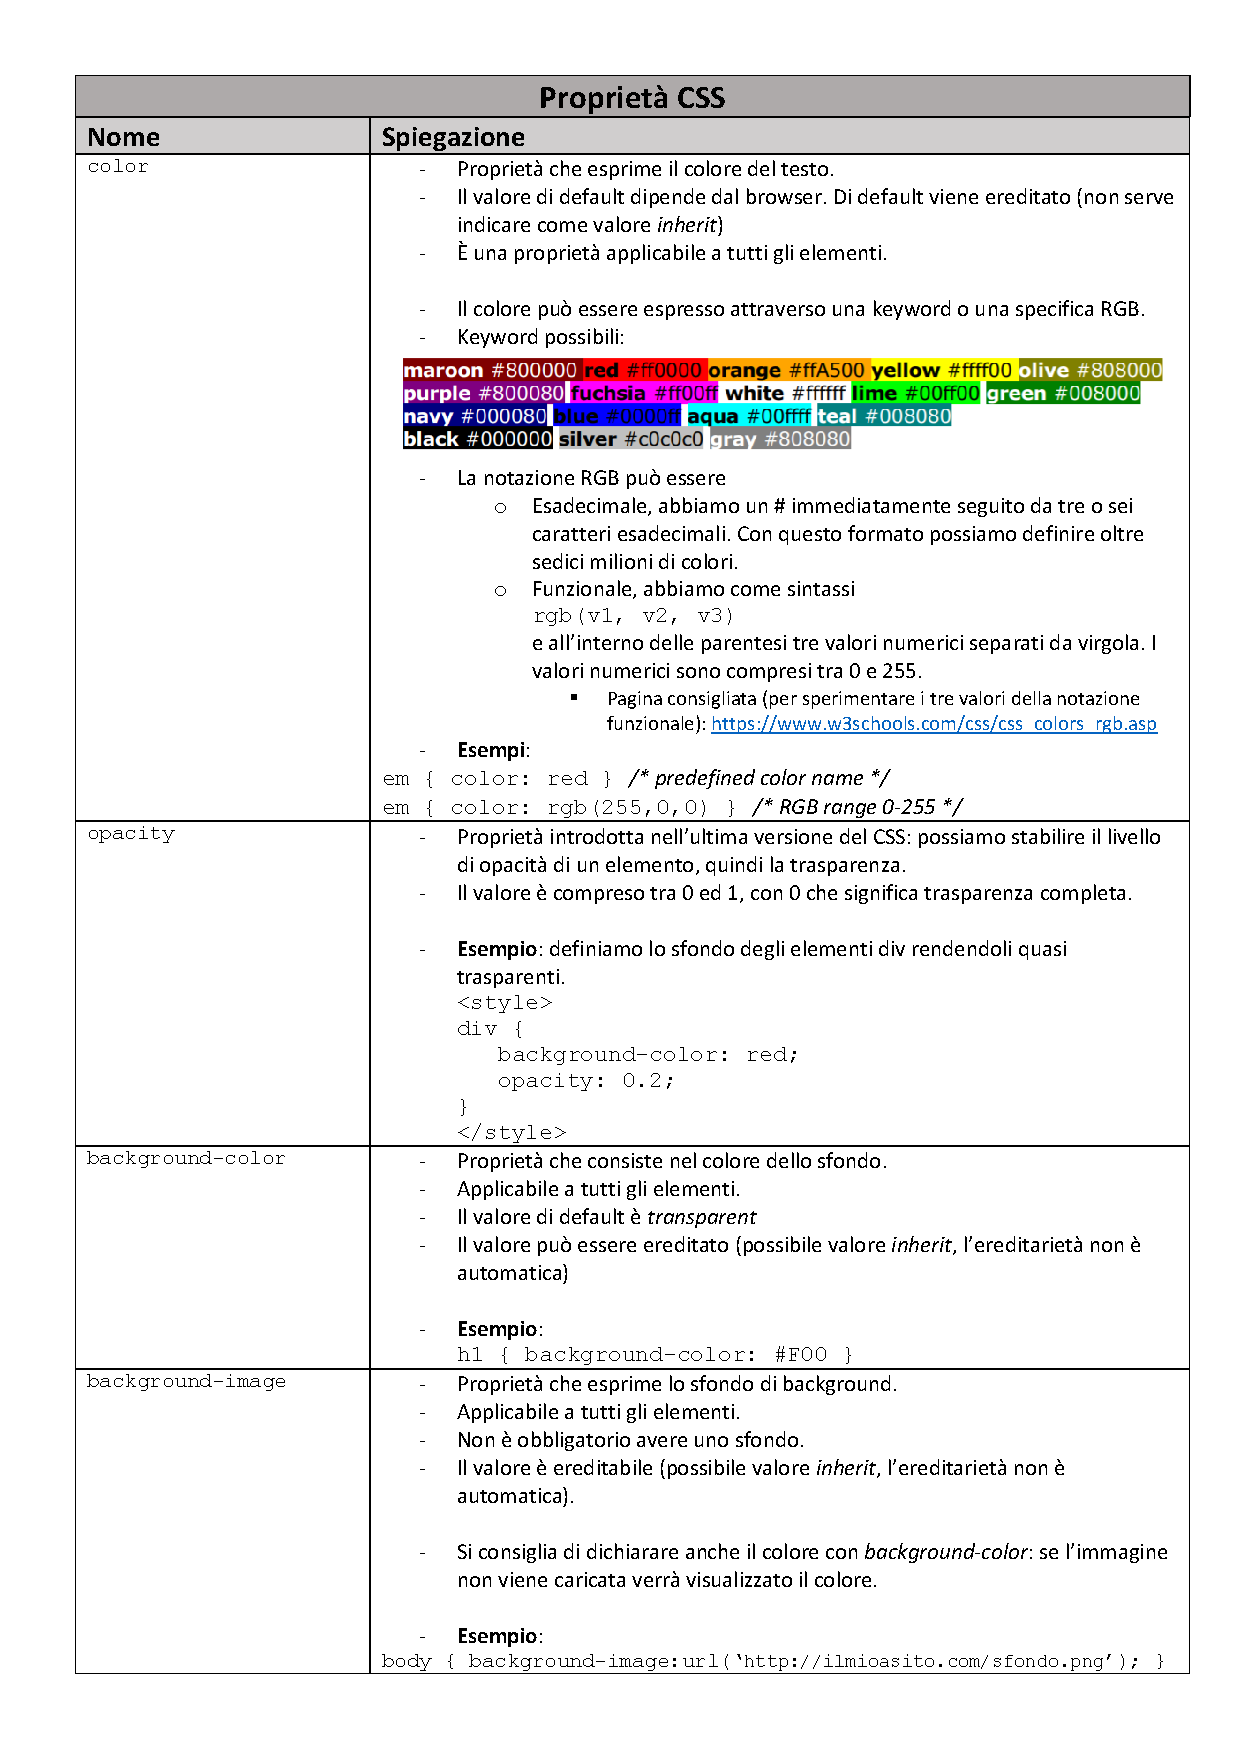
\includepdf[pagecommand={\thispagestyle{plain}},scale=0.92,pages=-]{pdf/css2}
 
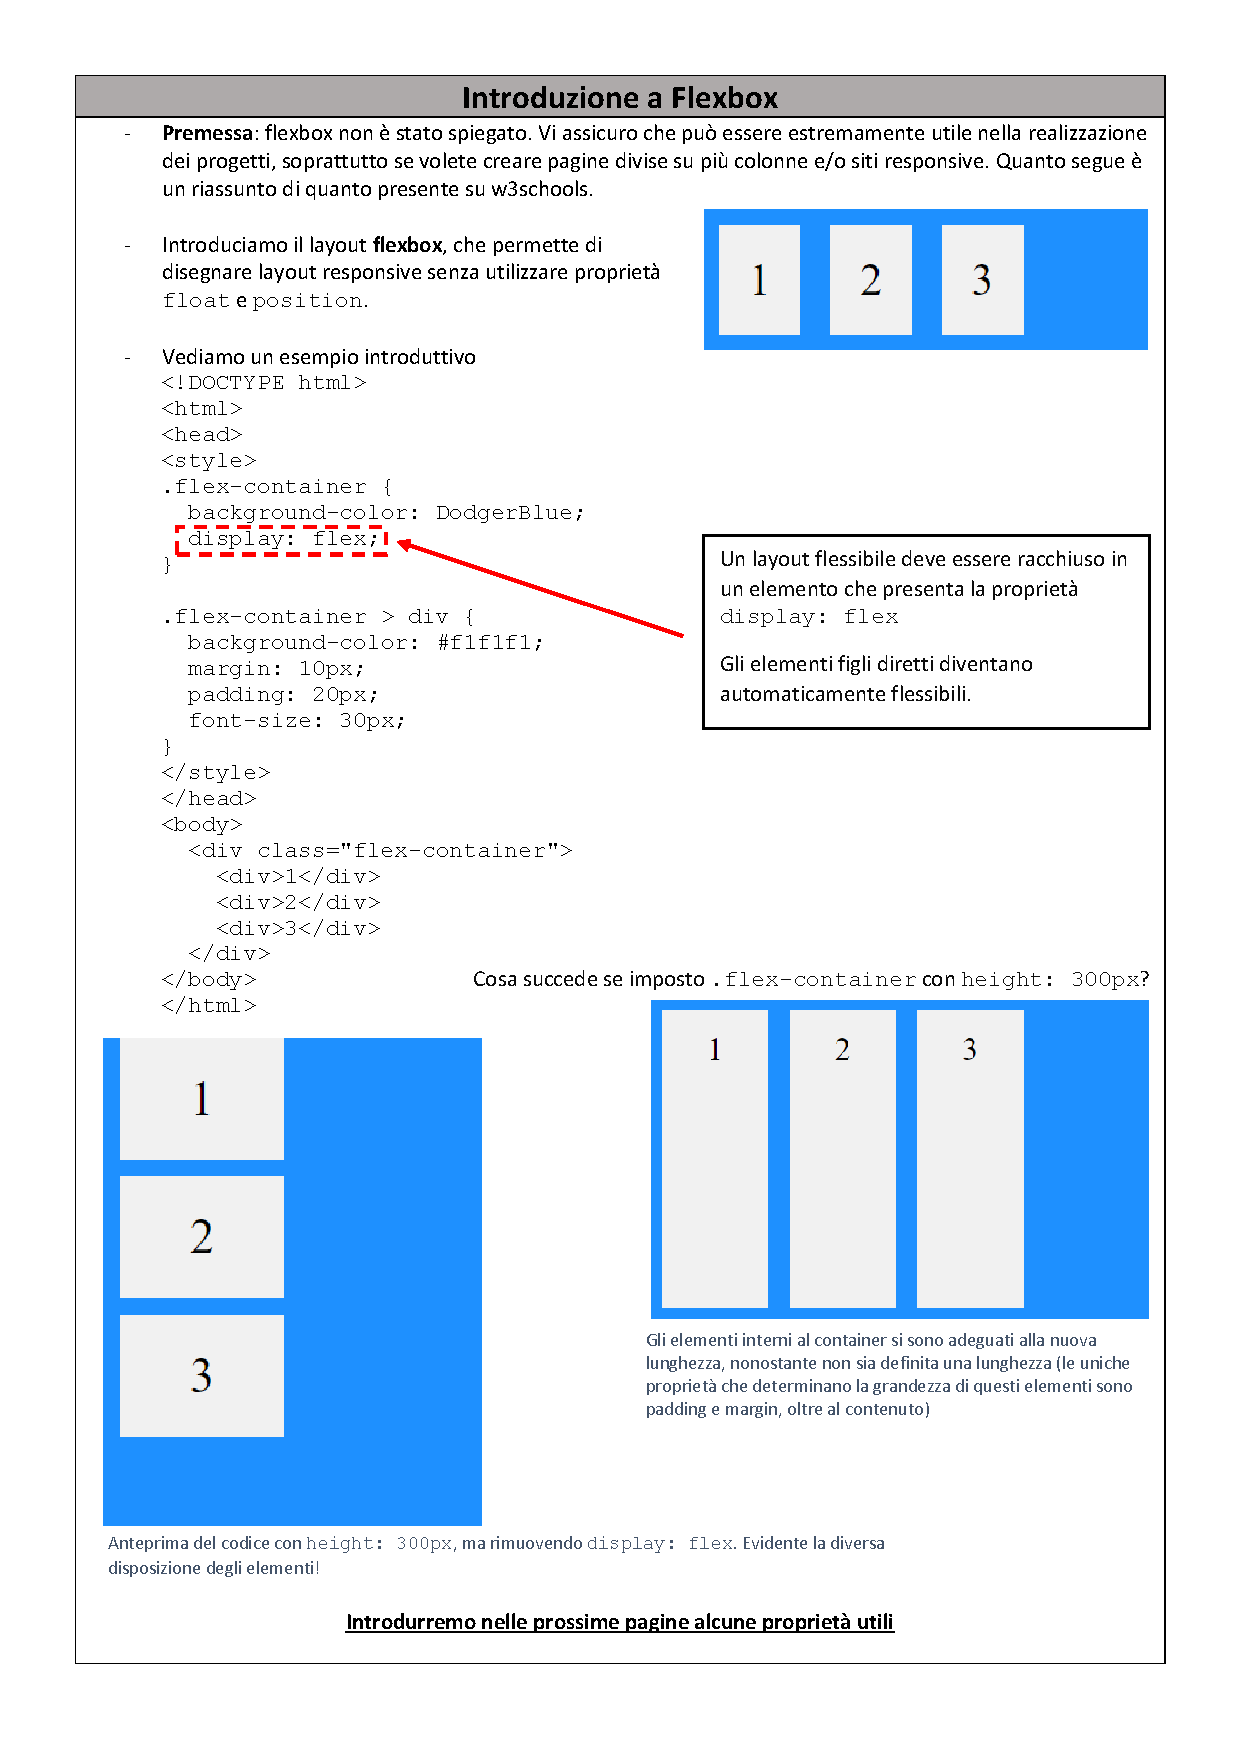
\includepdf[pagecommand={\thispagestyle{plain}},scale=0.92,pages=-]{pdf/flexbox}

\chapter{Javascript}
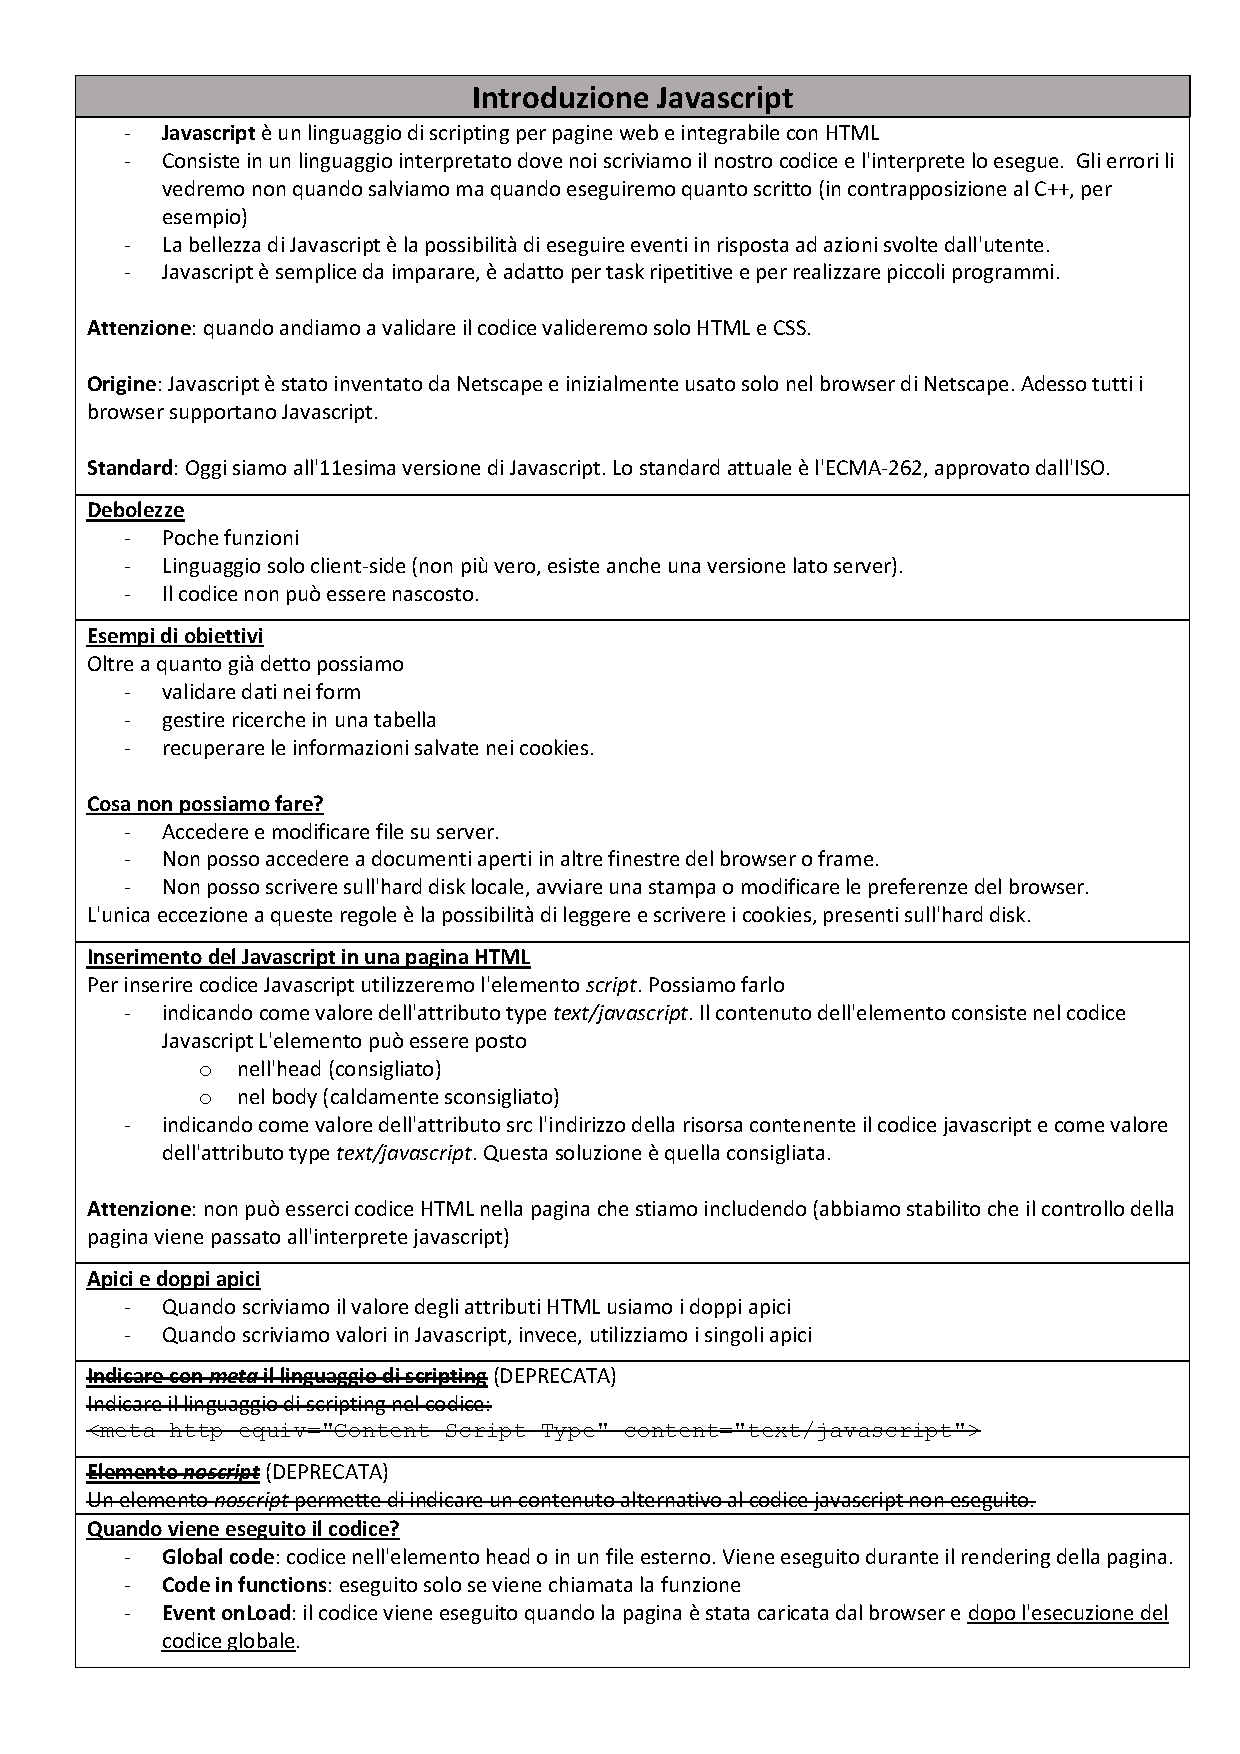
\includepdf[pagecommand={\thispagestyle{plain}},scale=0.92,pages=-]{pdf/javascript}
 
\chapter{PHP}
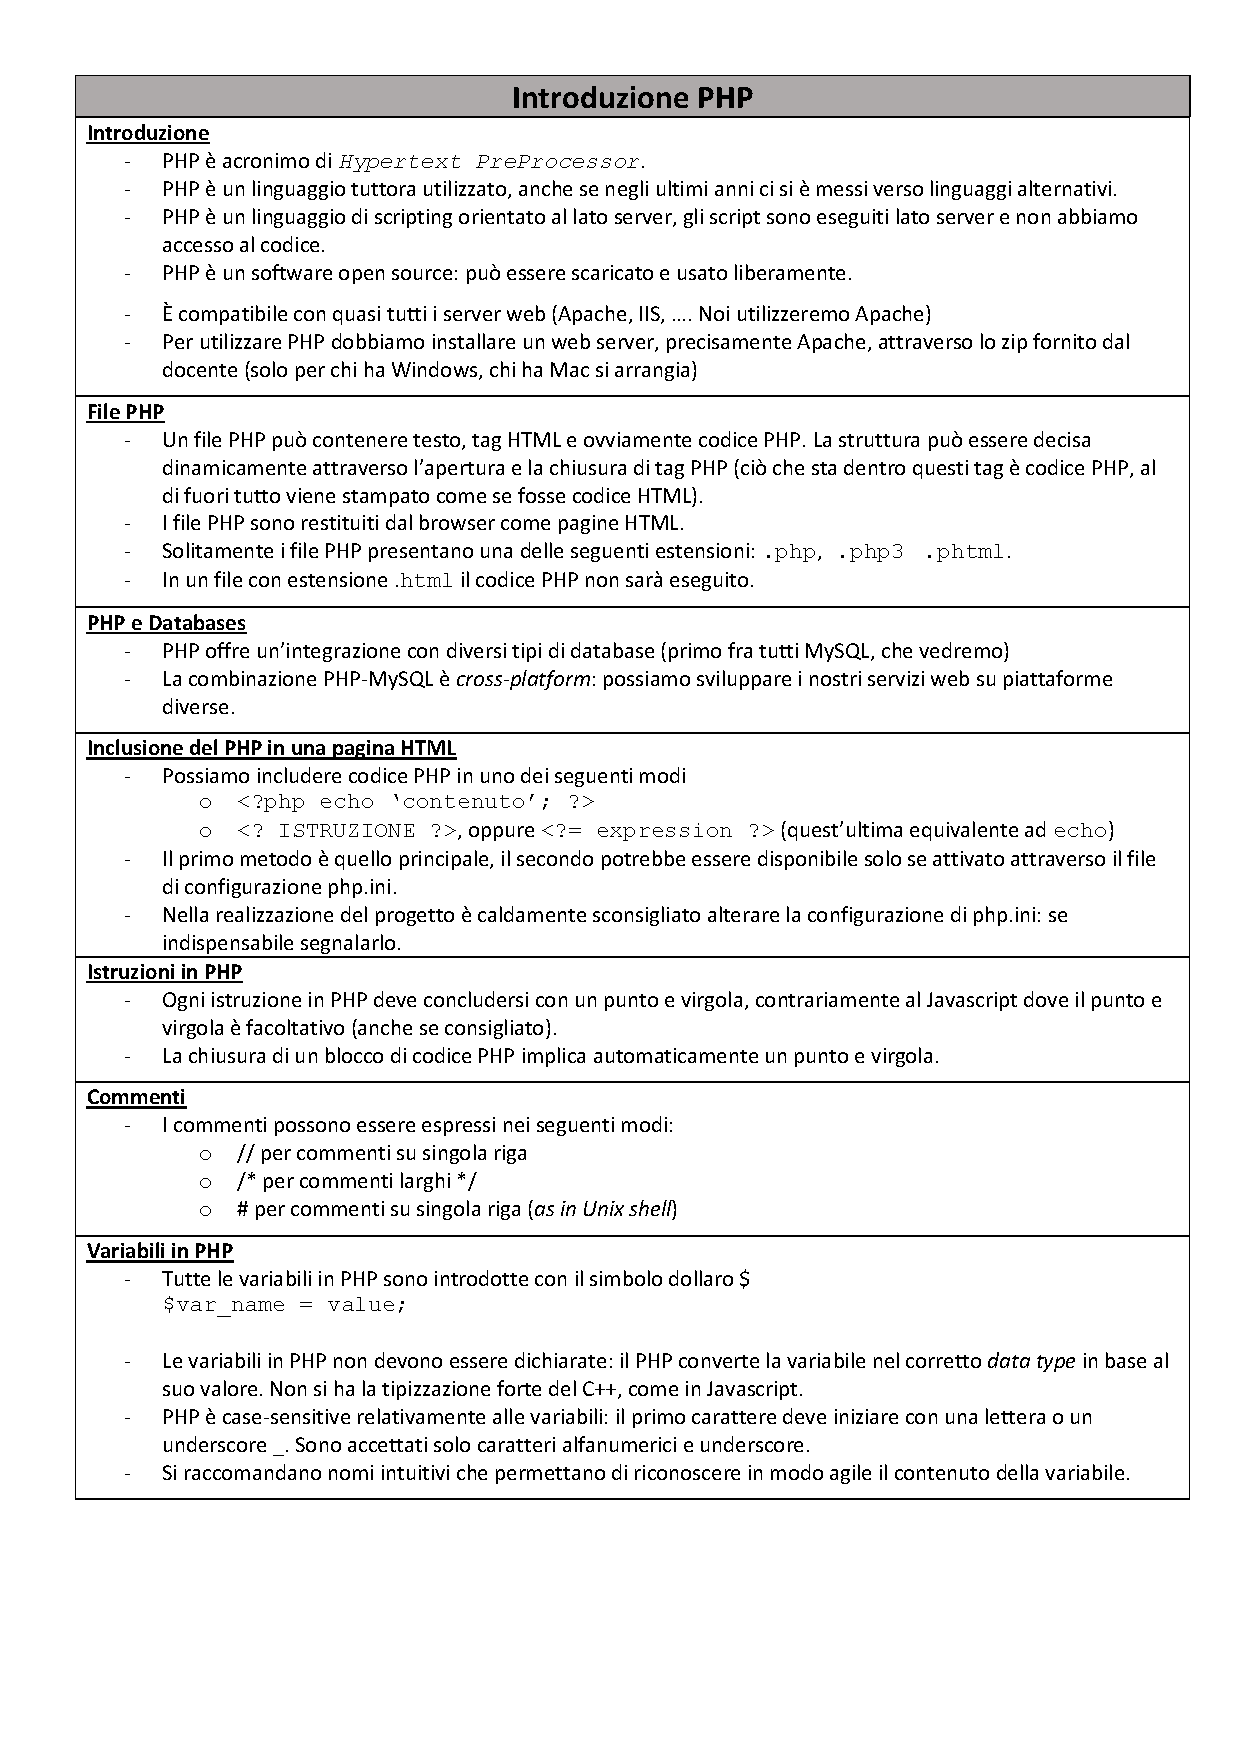
\includepdf[pagecommand={\thispagestyle{plain}},scale=0.92,pages=-]{pdf/php}
\chapter{HTTP}
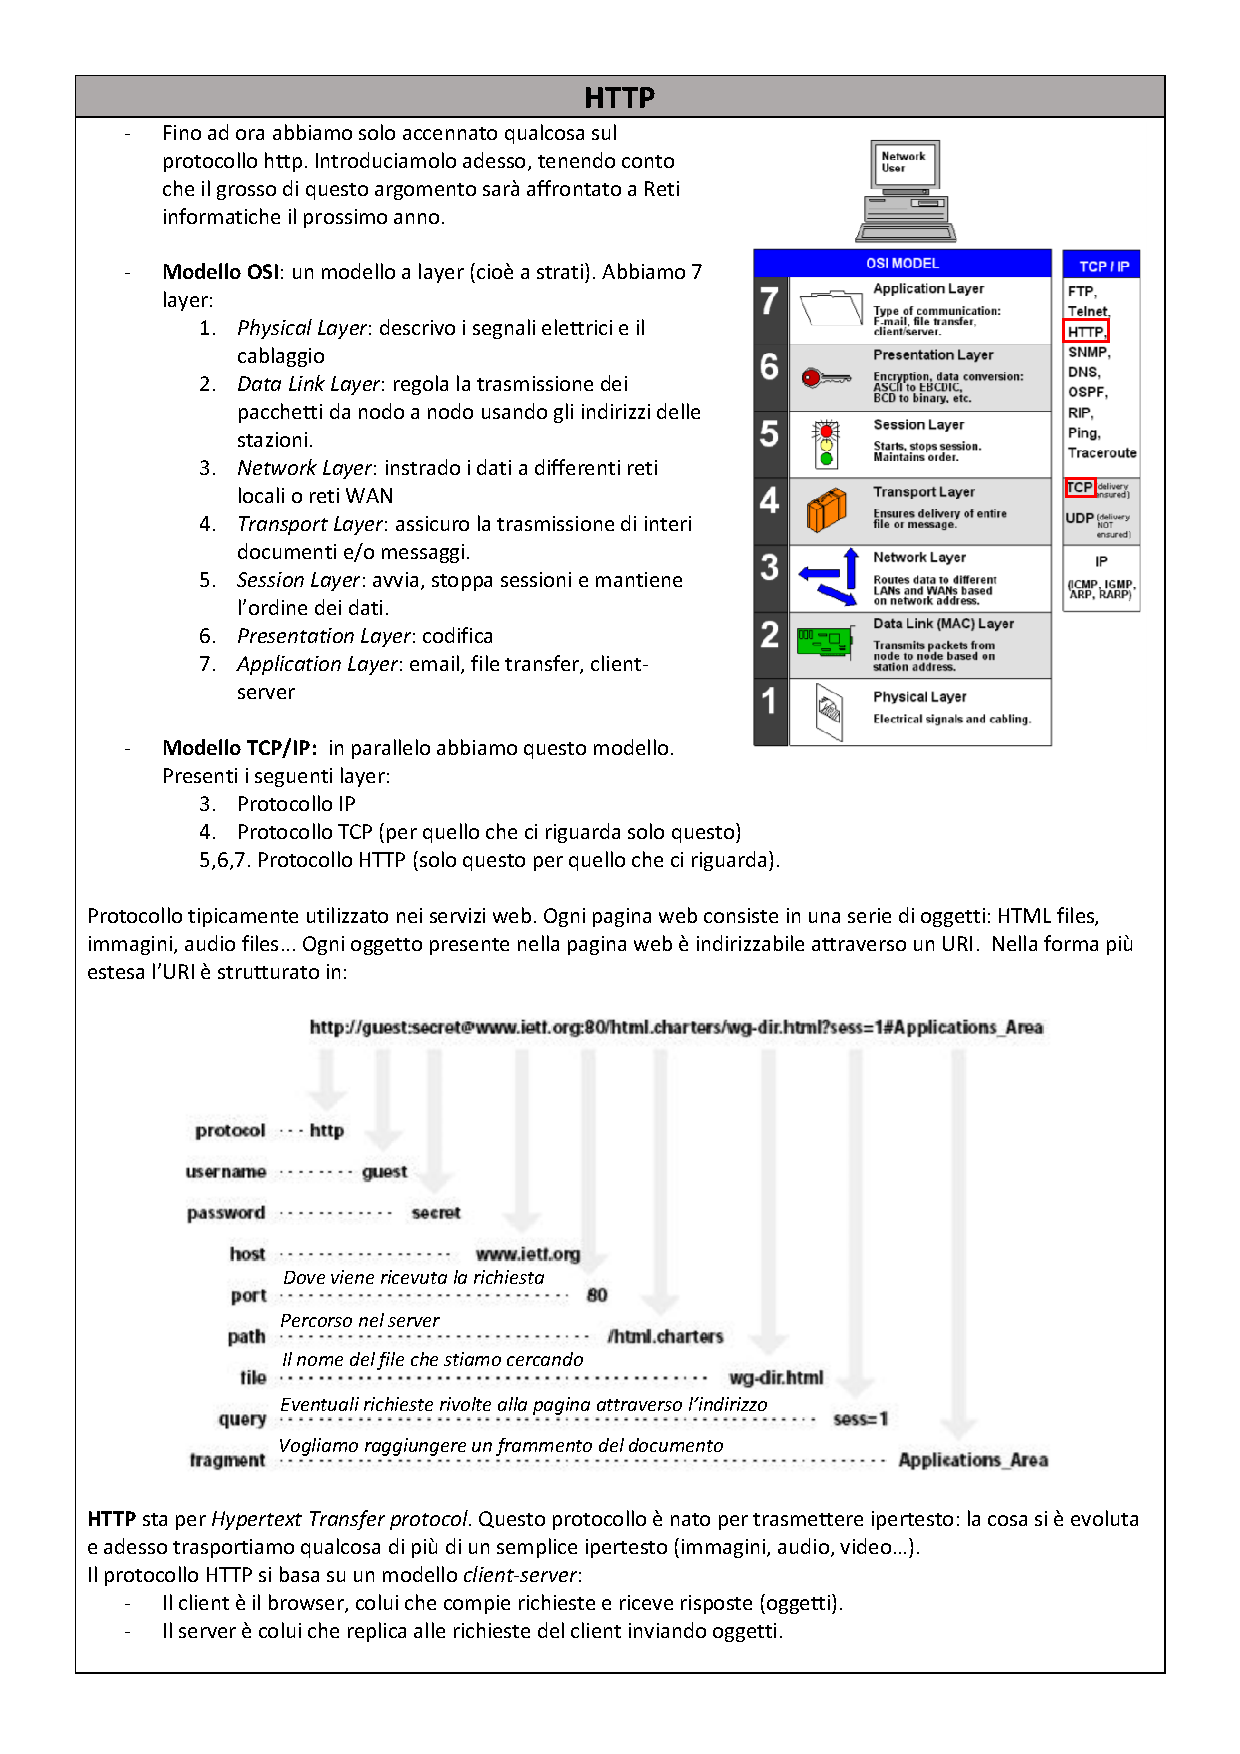
\includepdf[pagecommand={\thispagestyle{plain}},scale=0.92,pages=-]{pdf/HTTP}
 
 
\part{Esercitazioni di Tesconi}
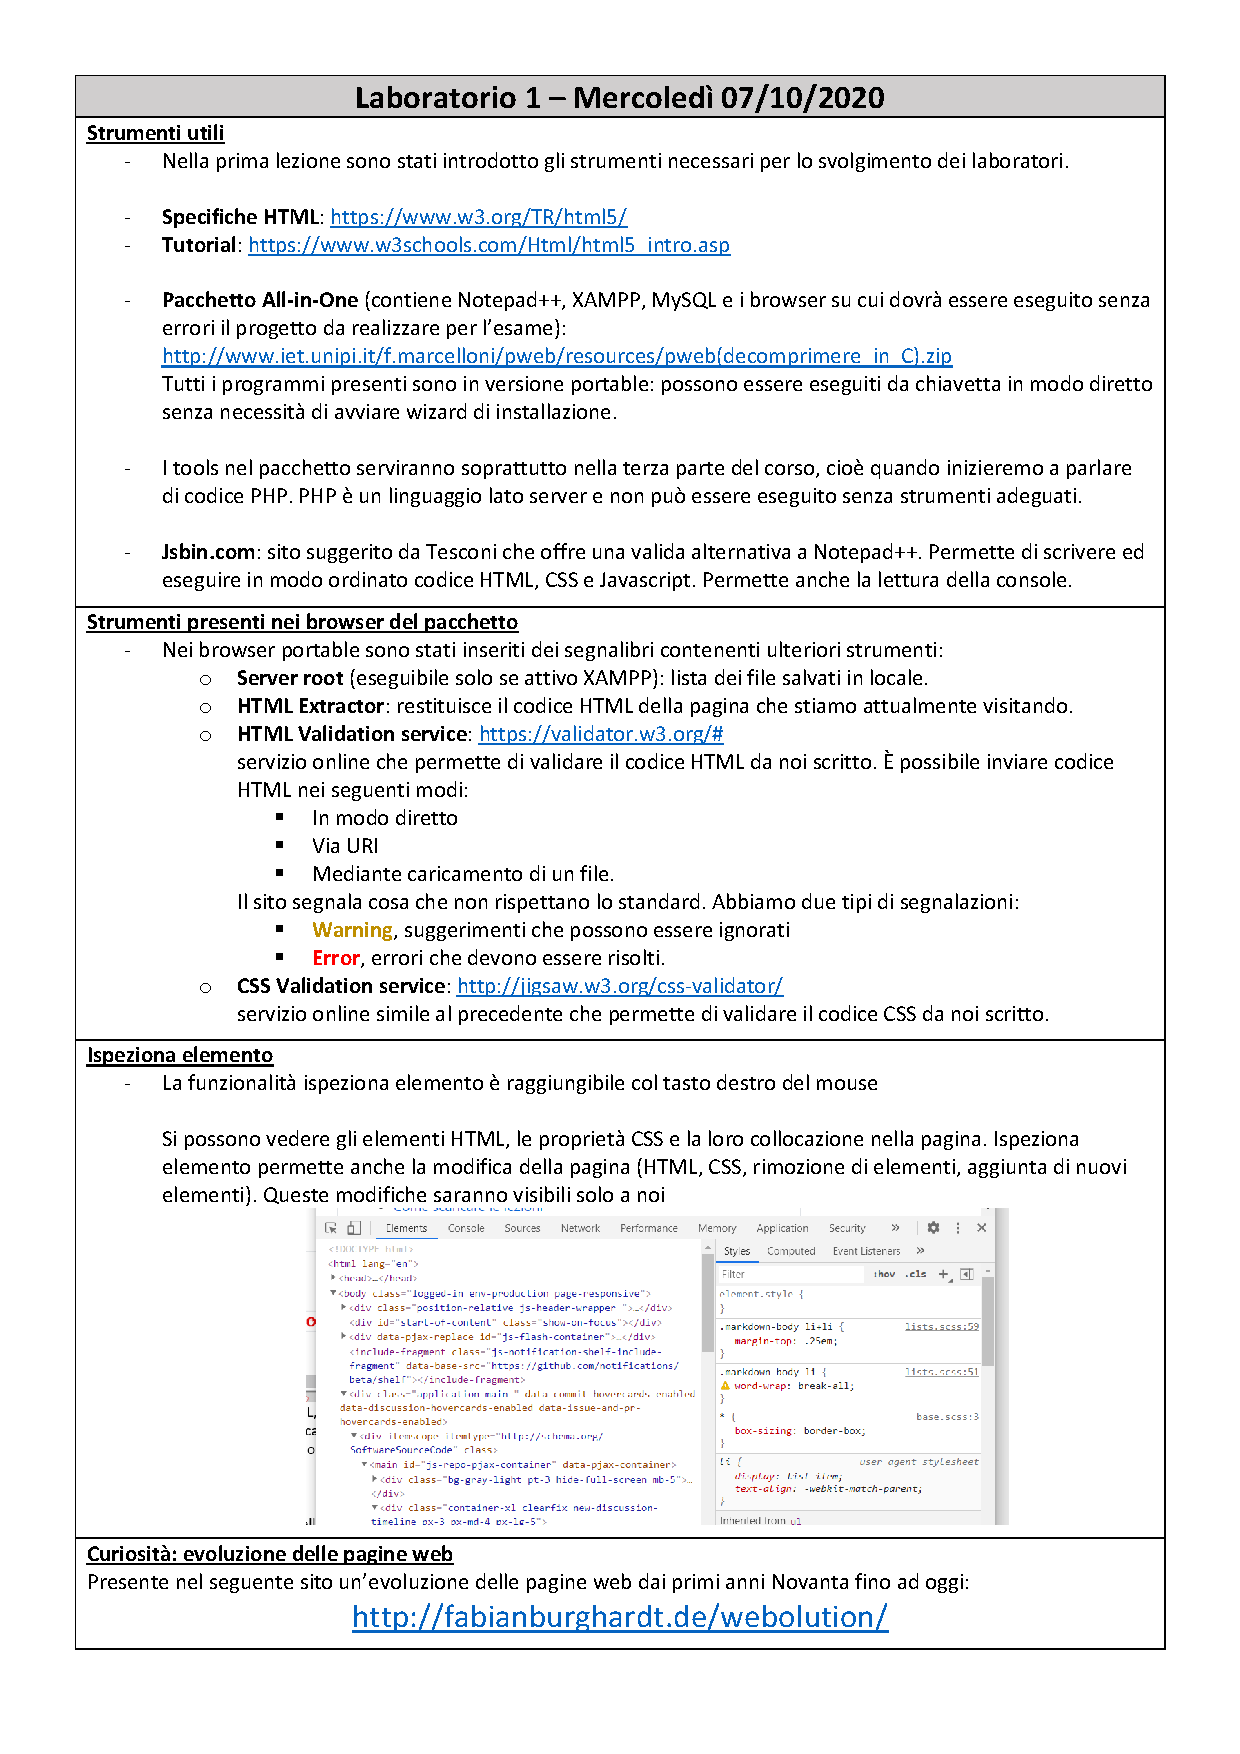
\includepdf[pagecommand={\thispagestyle{plain}},addtotoc={1,chapter,1,{Lab 1 - Mercoledì 07/10/2020},p1},scale=0.92,pages=-]{pdf/lab1}
\includepdf[pagecommand={\thispagestyle{plain}},nup=2x3,frame,scale=0.85,pages=-]{pdf/lab1diap}
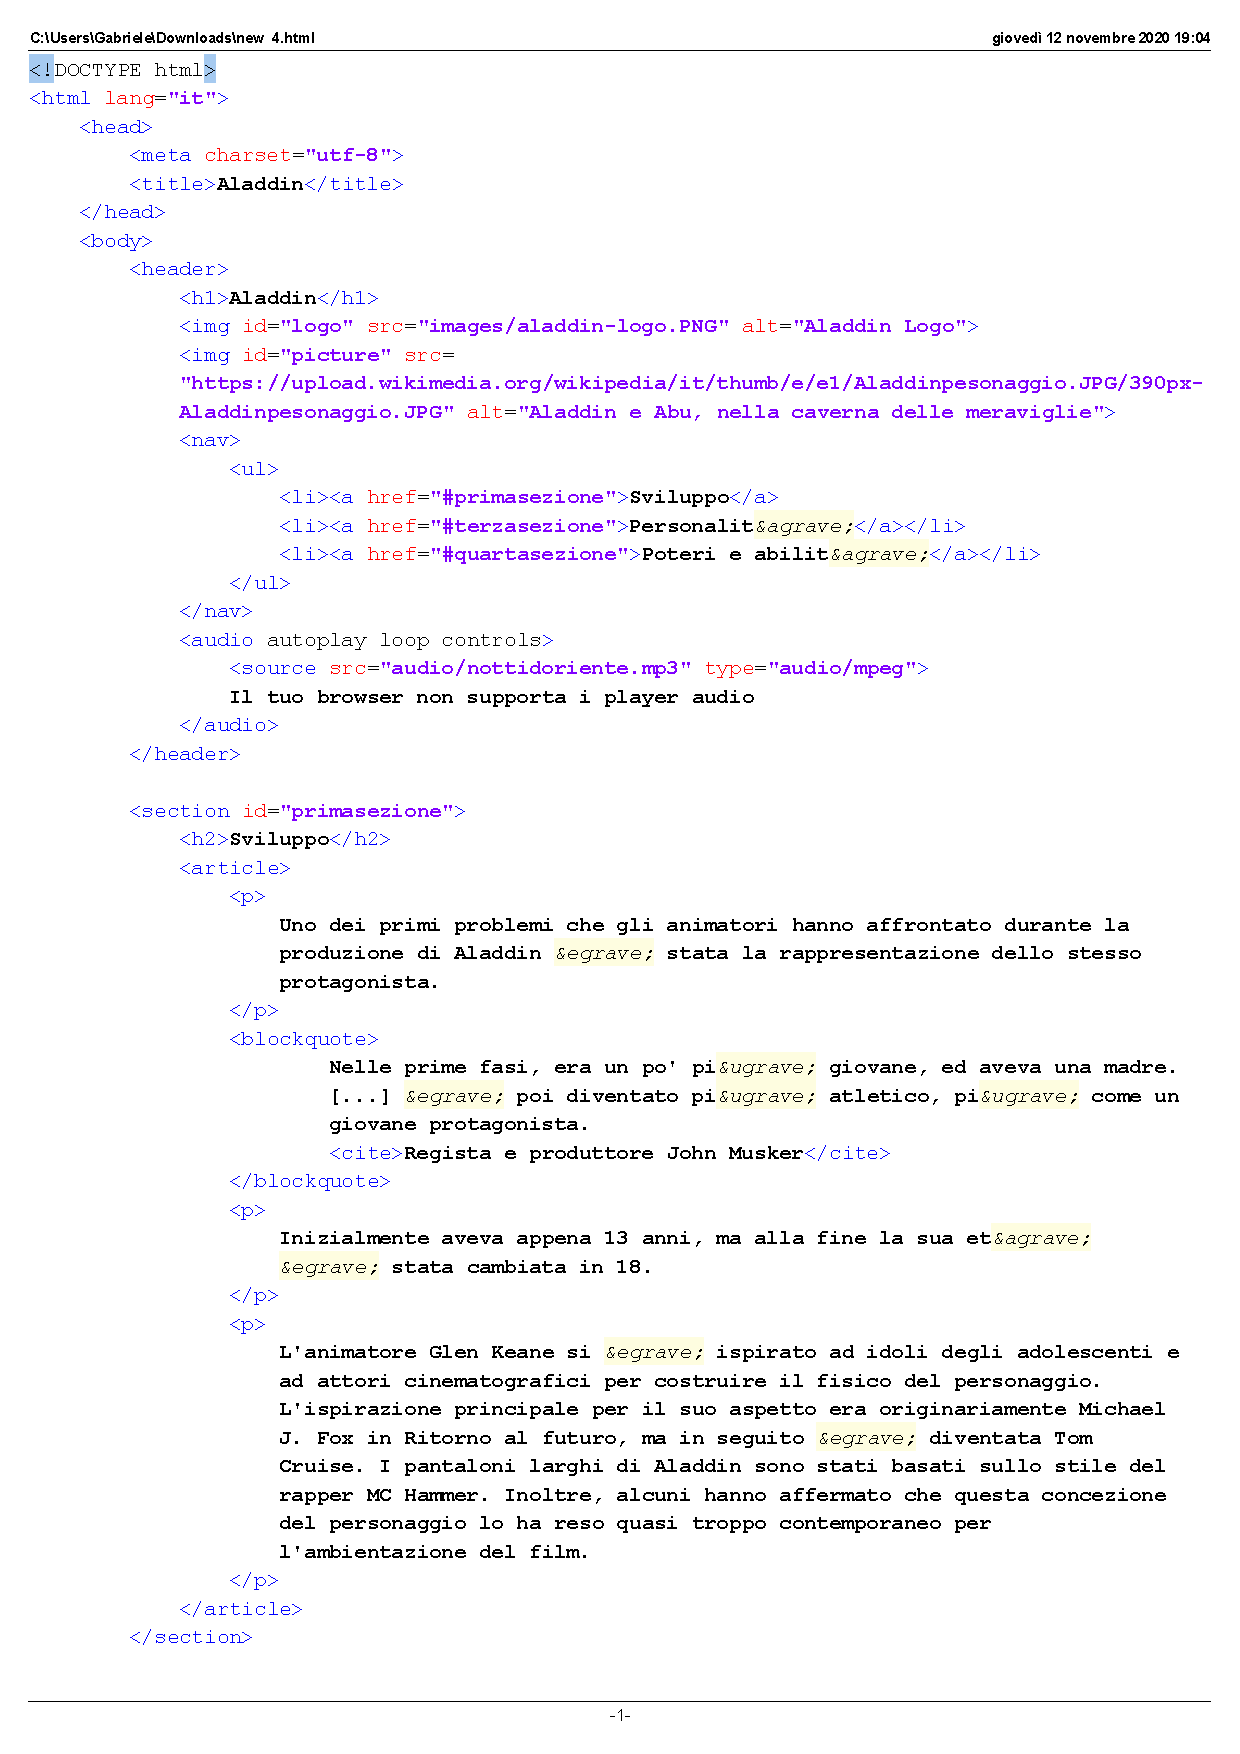
\includepdf[pagecommand={\thispagestyle{plain}},scale=0.85,pages=-]{pdf/lab1escasa}
\begin{center}
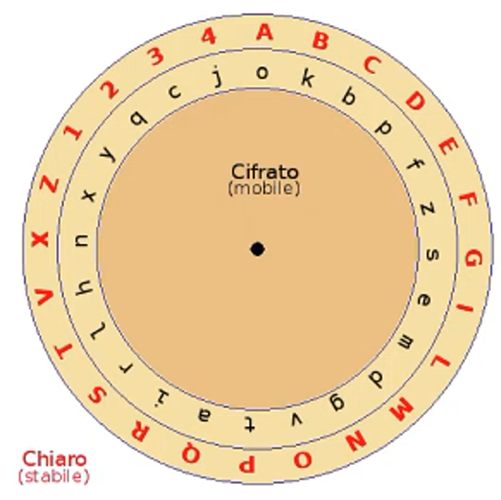
\includegraphics[scale=0.4]{img/8.PNG}
\end{center}
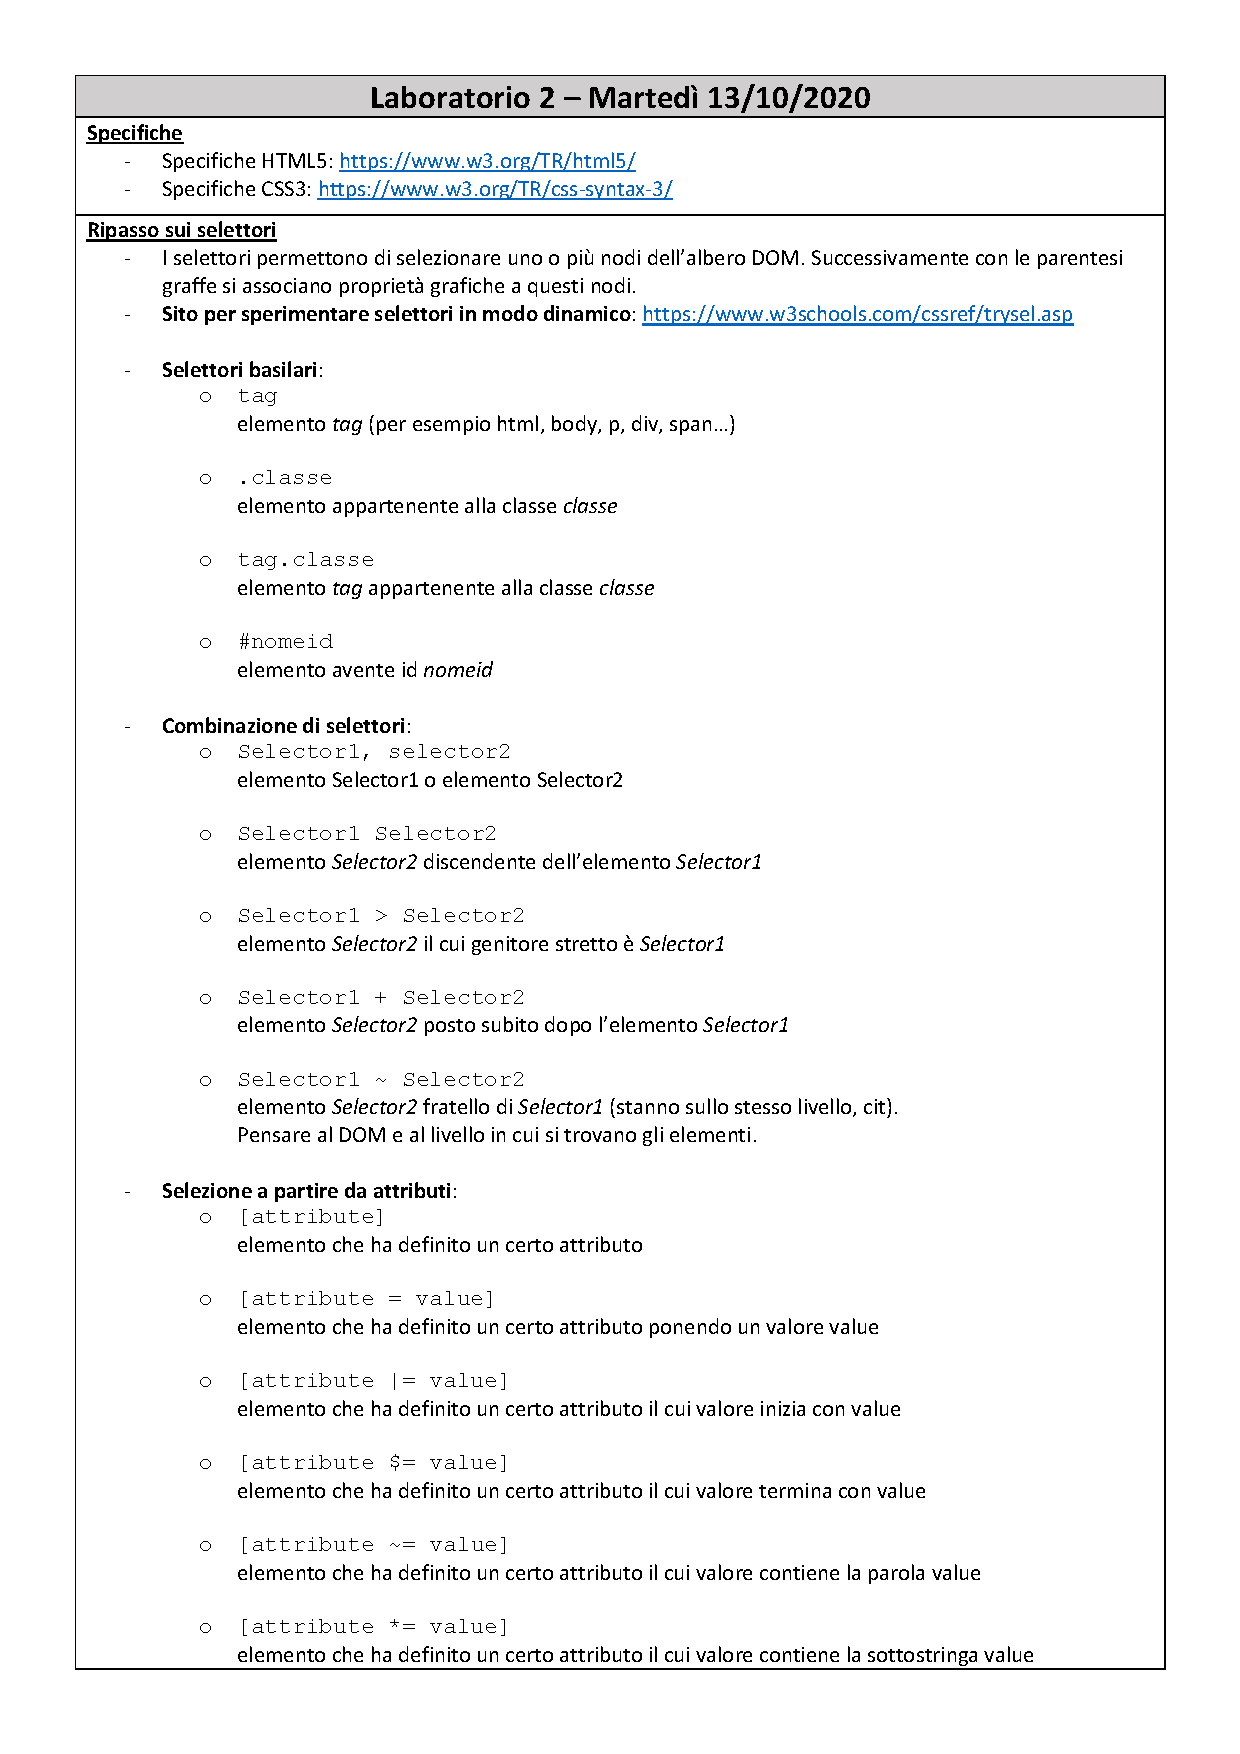
\includepdf[pagecommand={\thispagestyle{plain}},addtotoc={1,chapter,1,{Lab 2 - Martedì 13/10/2020},p2},scale=0.92,pages=-]{pdf/lab2}
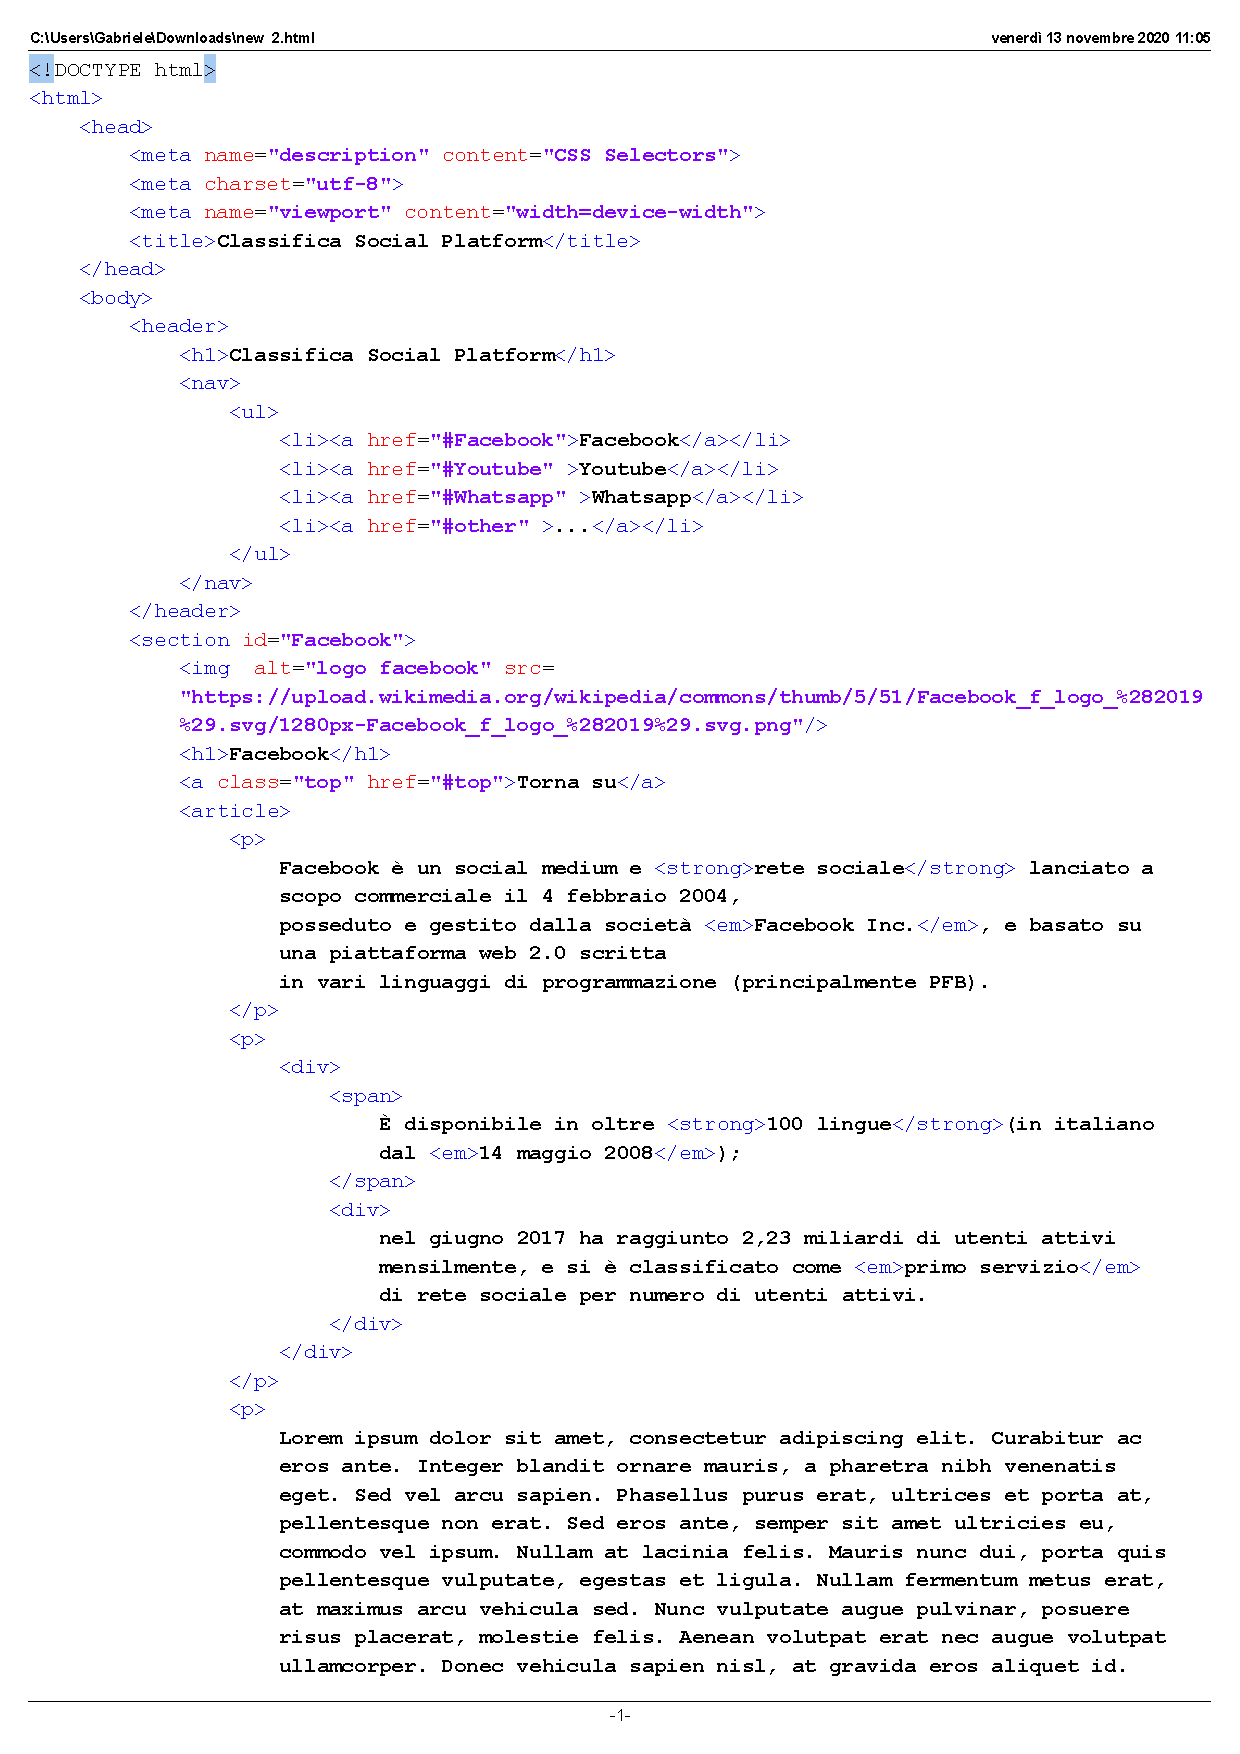
\includepdf[pagecommand={\thispagestyle{plain}},scale=0.85,pages=-]{pdf/lab2base}
\begin{center}
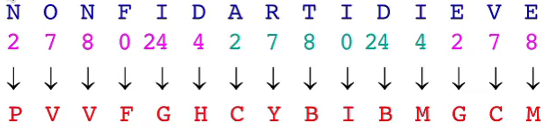
\includegraphics[scale=0.3]{img/9.PNG}
\thispagestyle{empty}
\end{center}
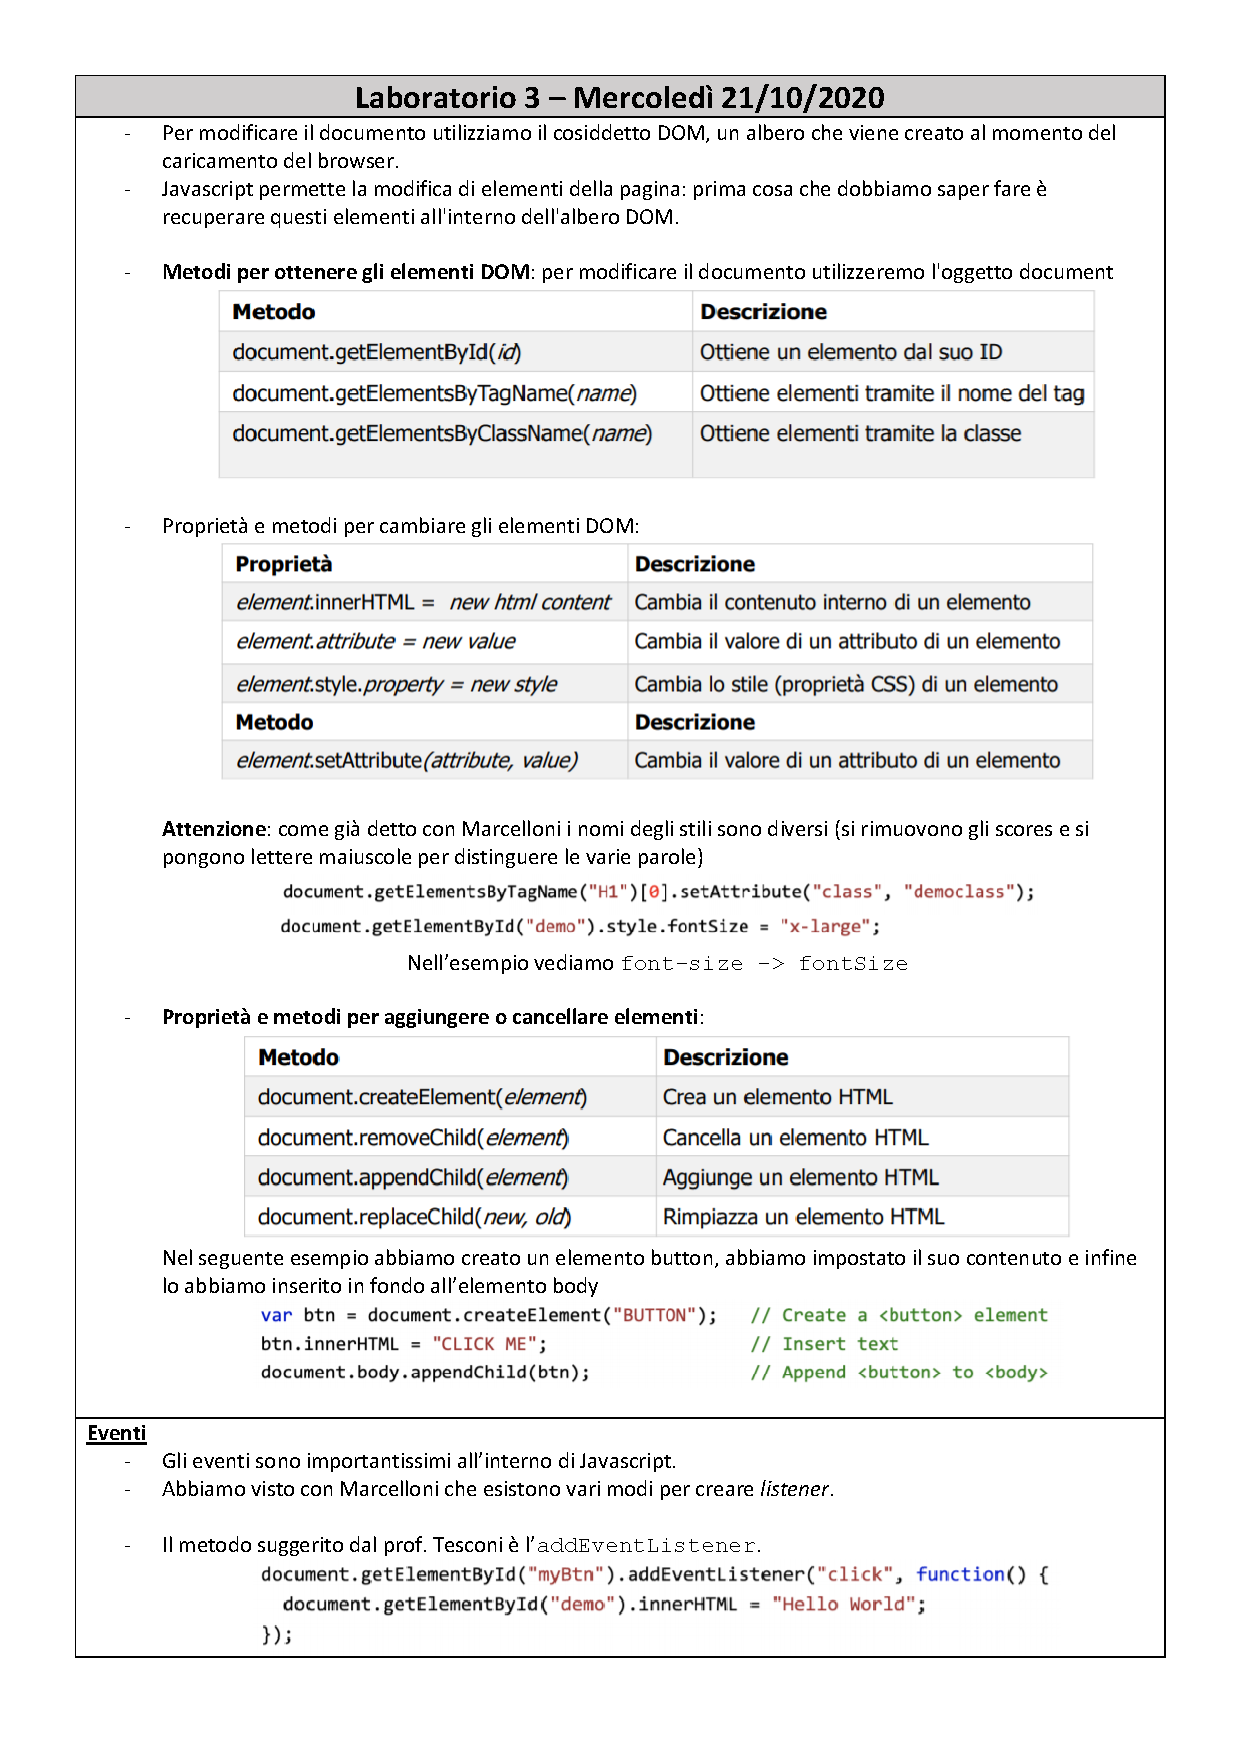
\includepdf[pagecommand={\thispagestyle{plain}},addtotoc={1,chapter,1,{Lab 3 - Mercoledì 21/10/2020},p3},scale=0.92,pages=-]{pdf/lab3}
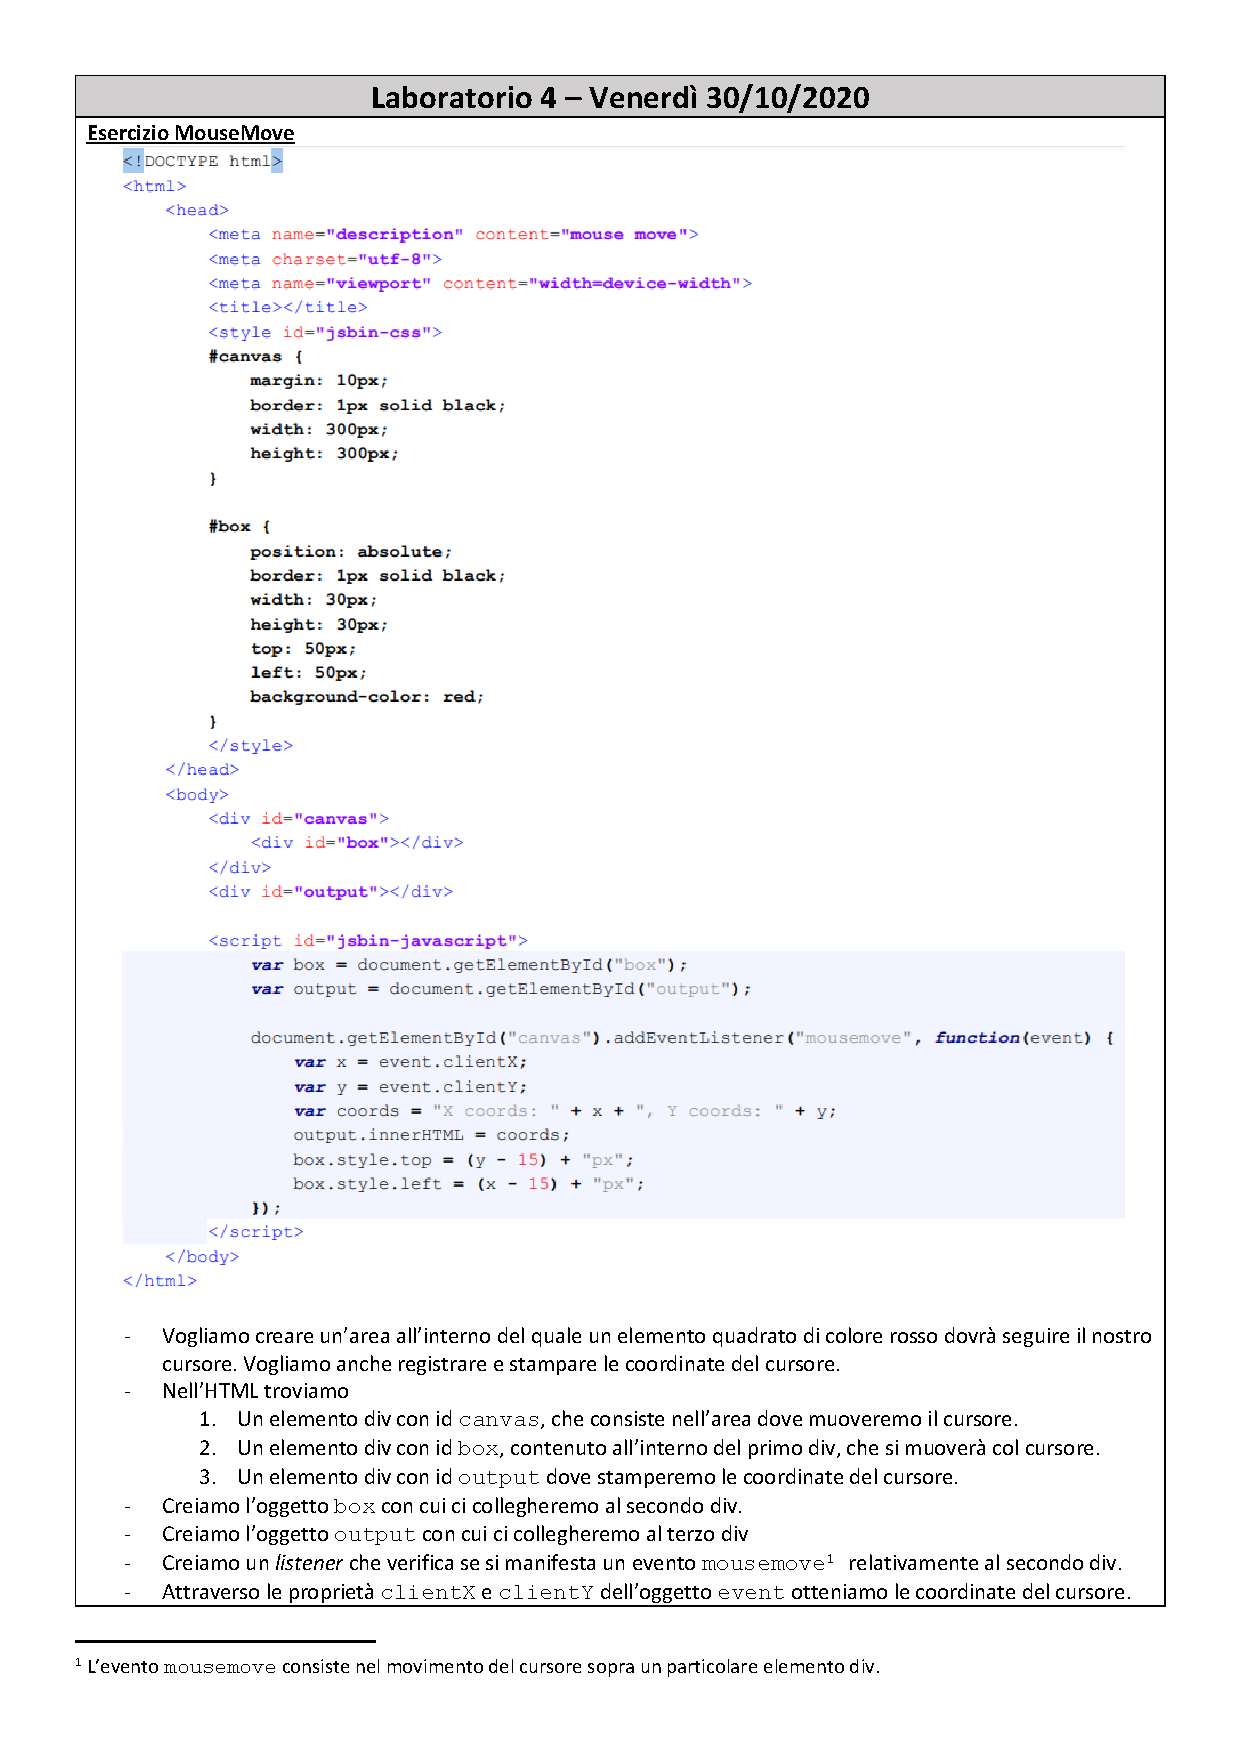
\includepdf[pagecommand={\thispagestyle{plain}},addtotoc={1,chapter,1,{Lab 4 - Venerdì 30/10/2020},p4},scale=0.92,pages=-]{pdf/lab4}
\begin{center}
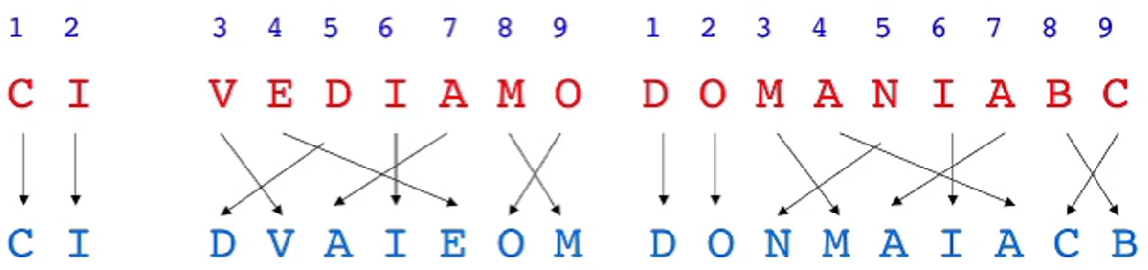
\includegraphics[scale=0.4]{img/10.PNG}
\end{center}
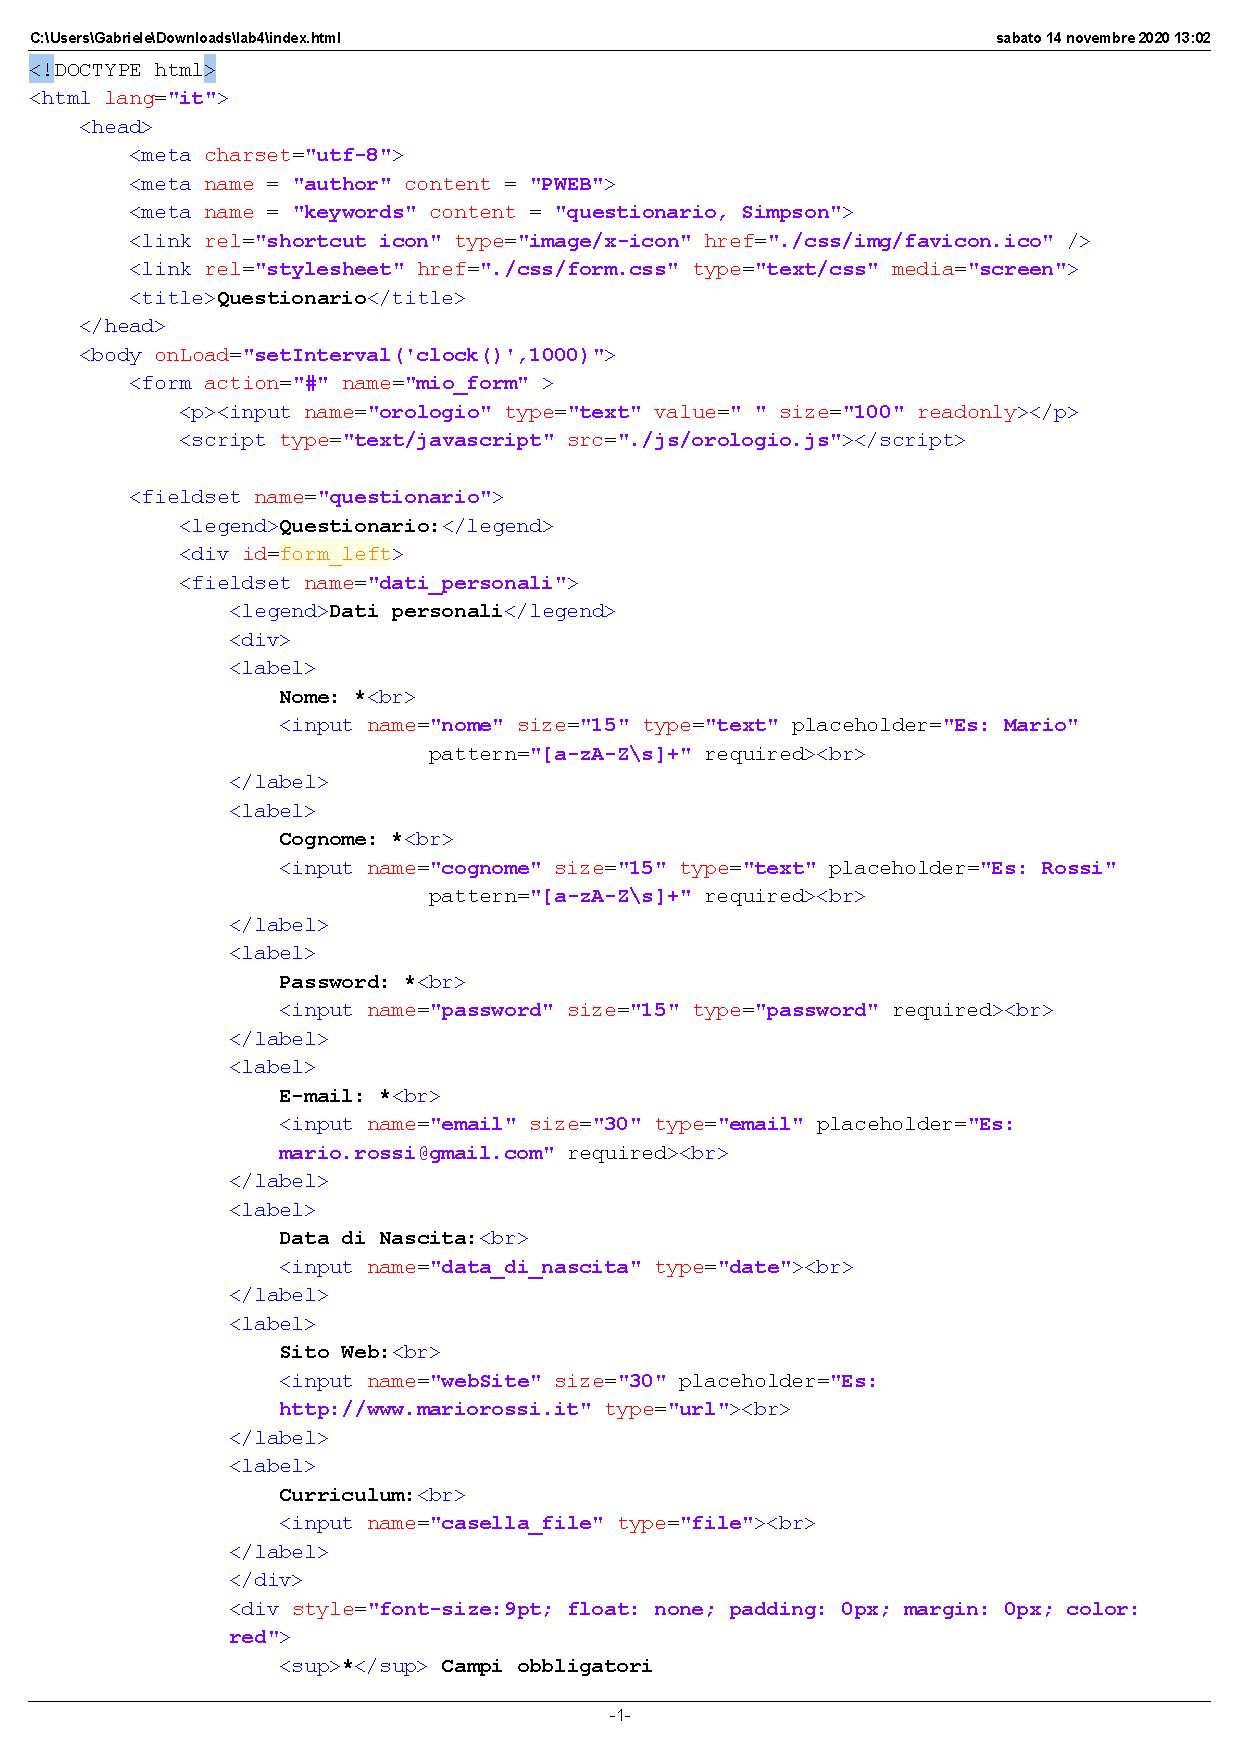
\includepdf[pagecommand={\thispagestyle{plain}},scale=0.85,pages=-]{pdf/lab4indexhtml}
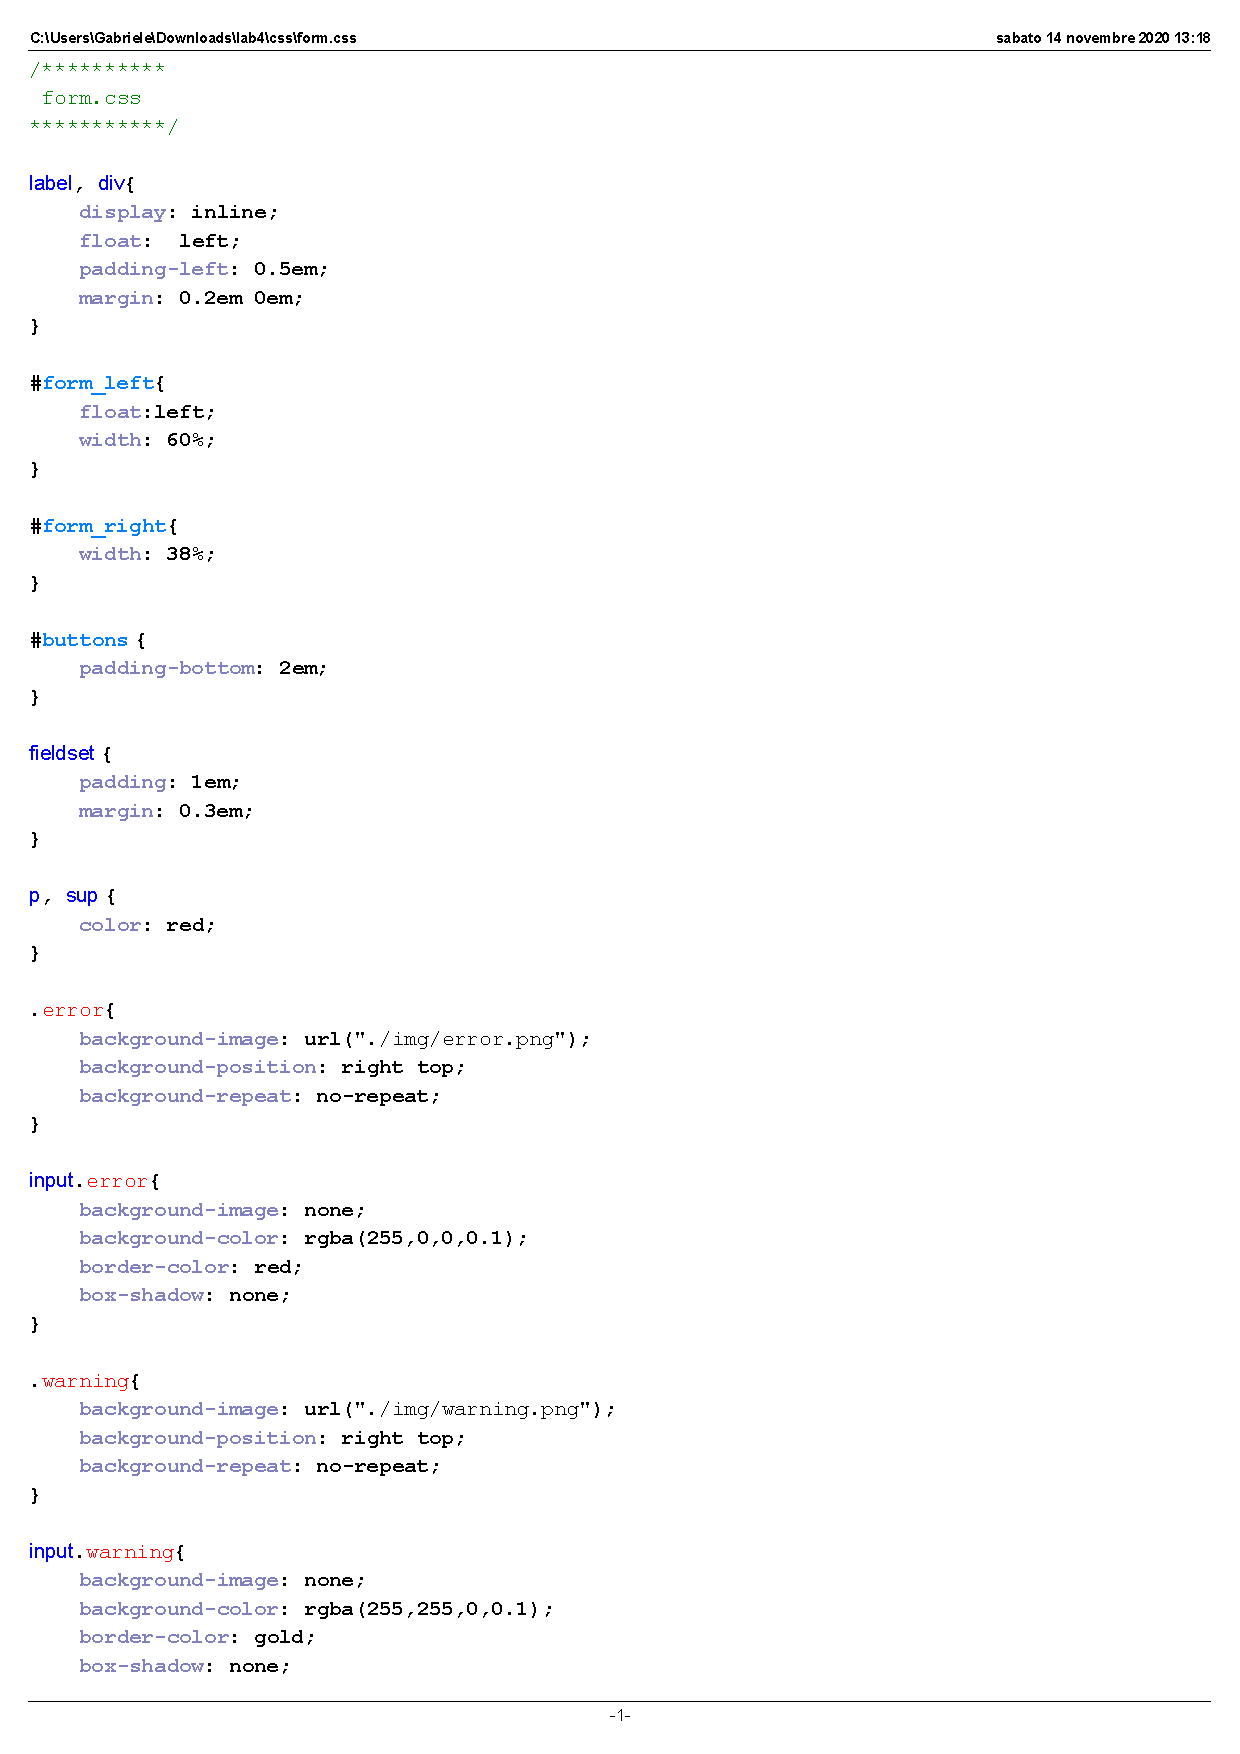
\includepdf[pagecommand={\thispagestyle{plain}},scale=0.85,pages=-]{pdf/lab4formcss}
  
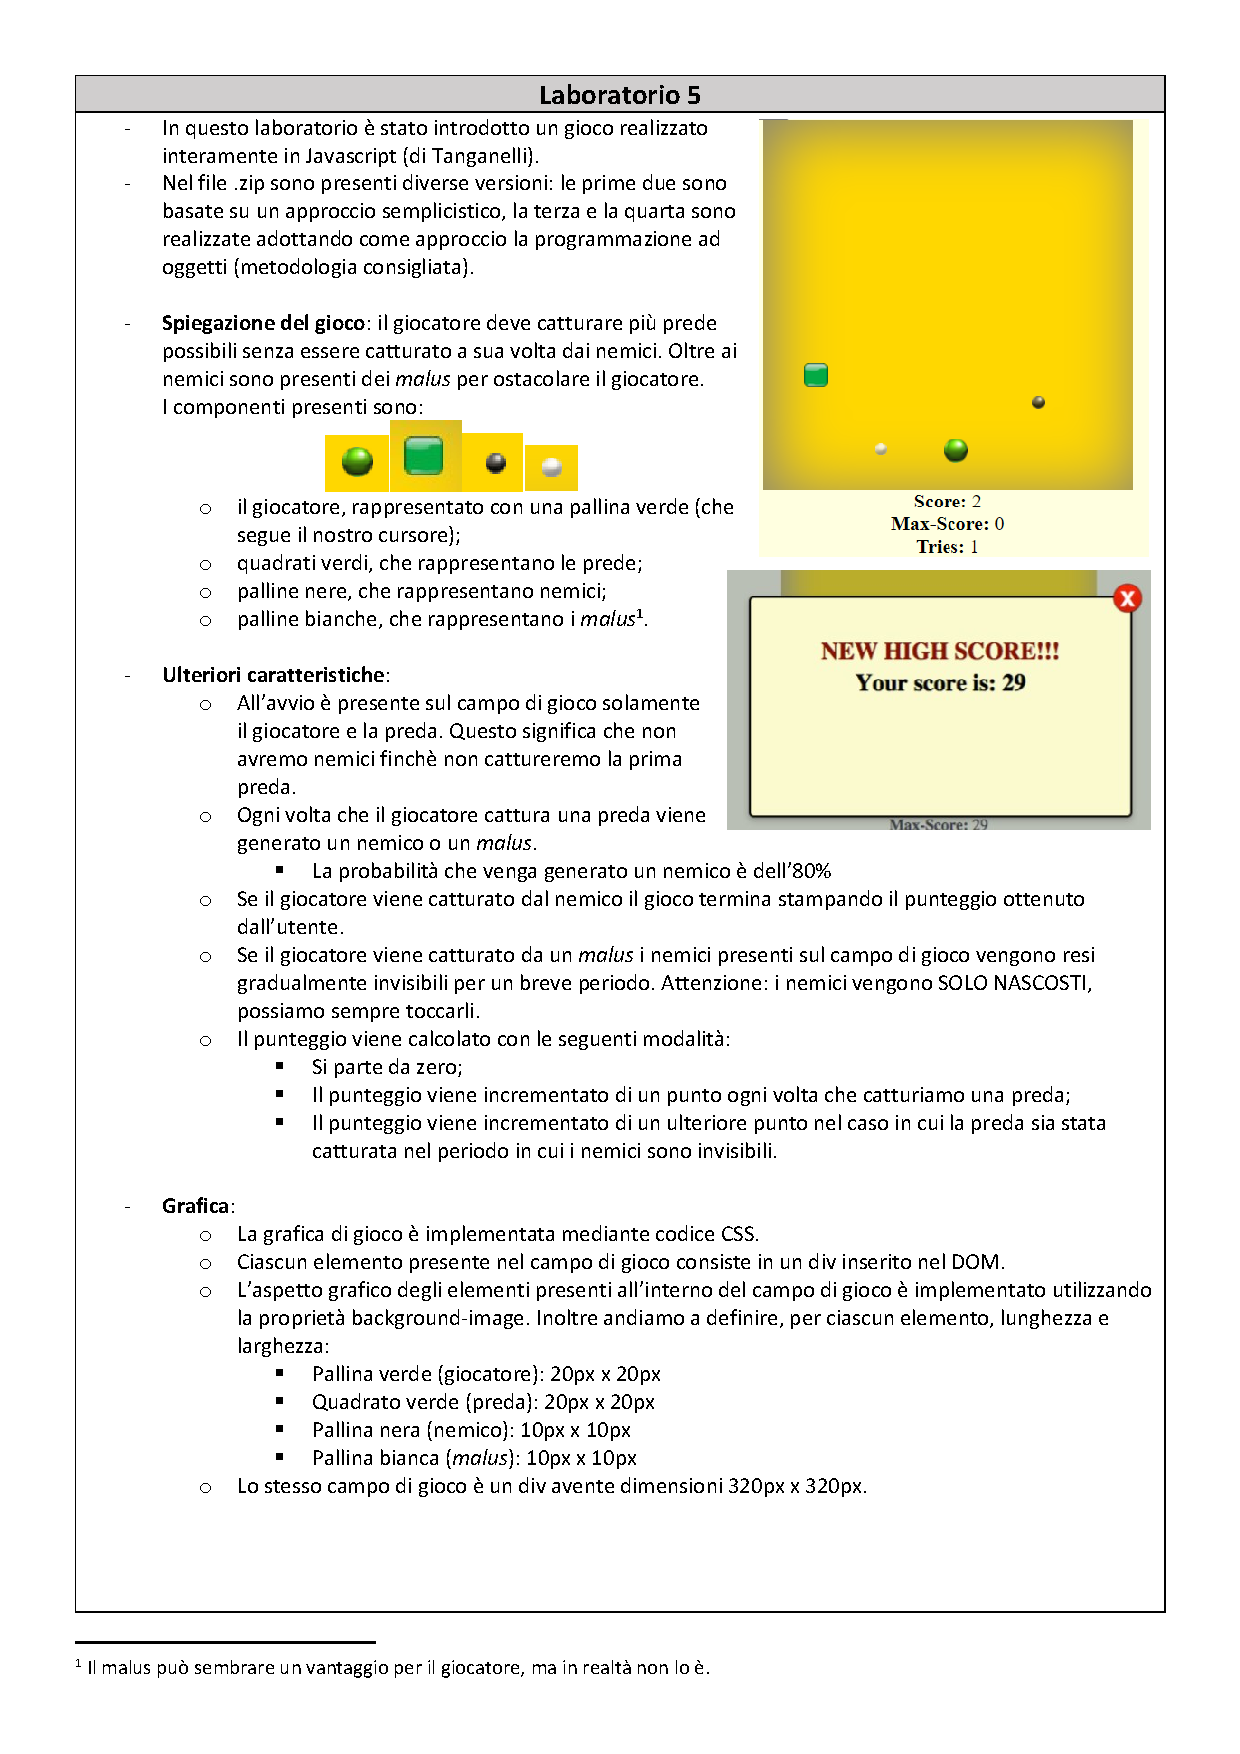
\includepdf[pagecommand={\thispagestyle{plain}},addtotoc={1,chapter,1,{Lab 5 - Martedì 03/11/2020},p4},scale=0.92,pages=-]{pdf/lab5}
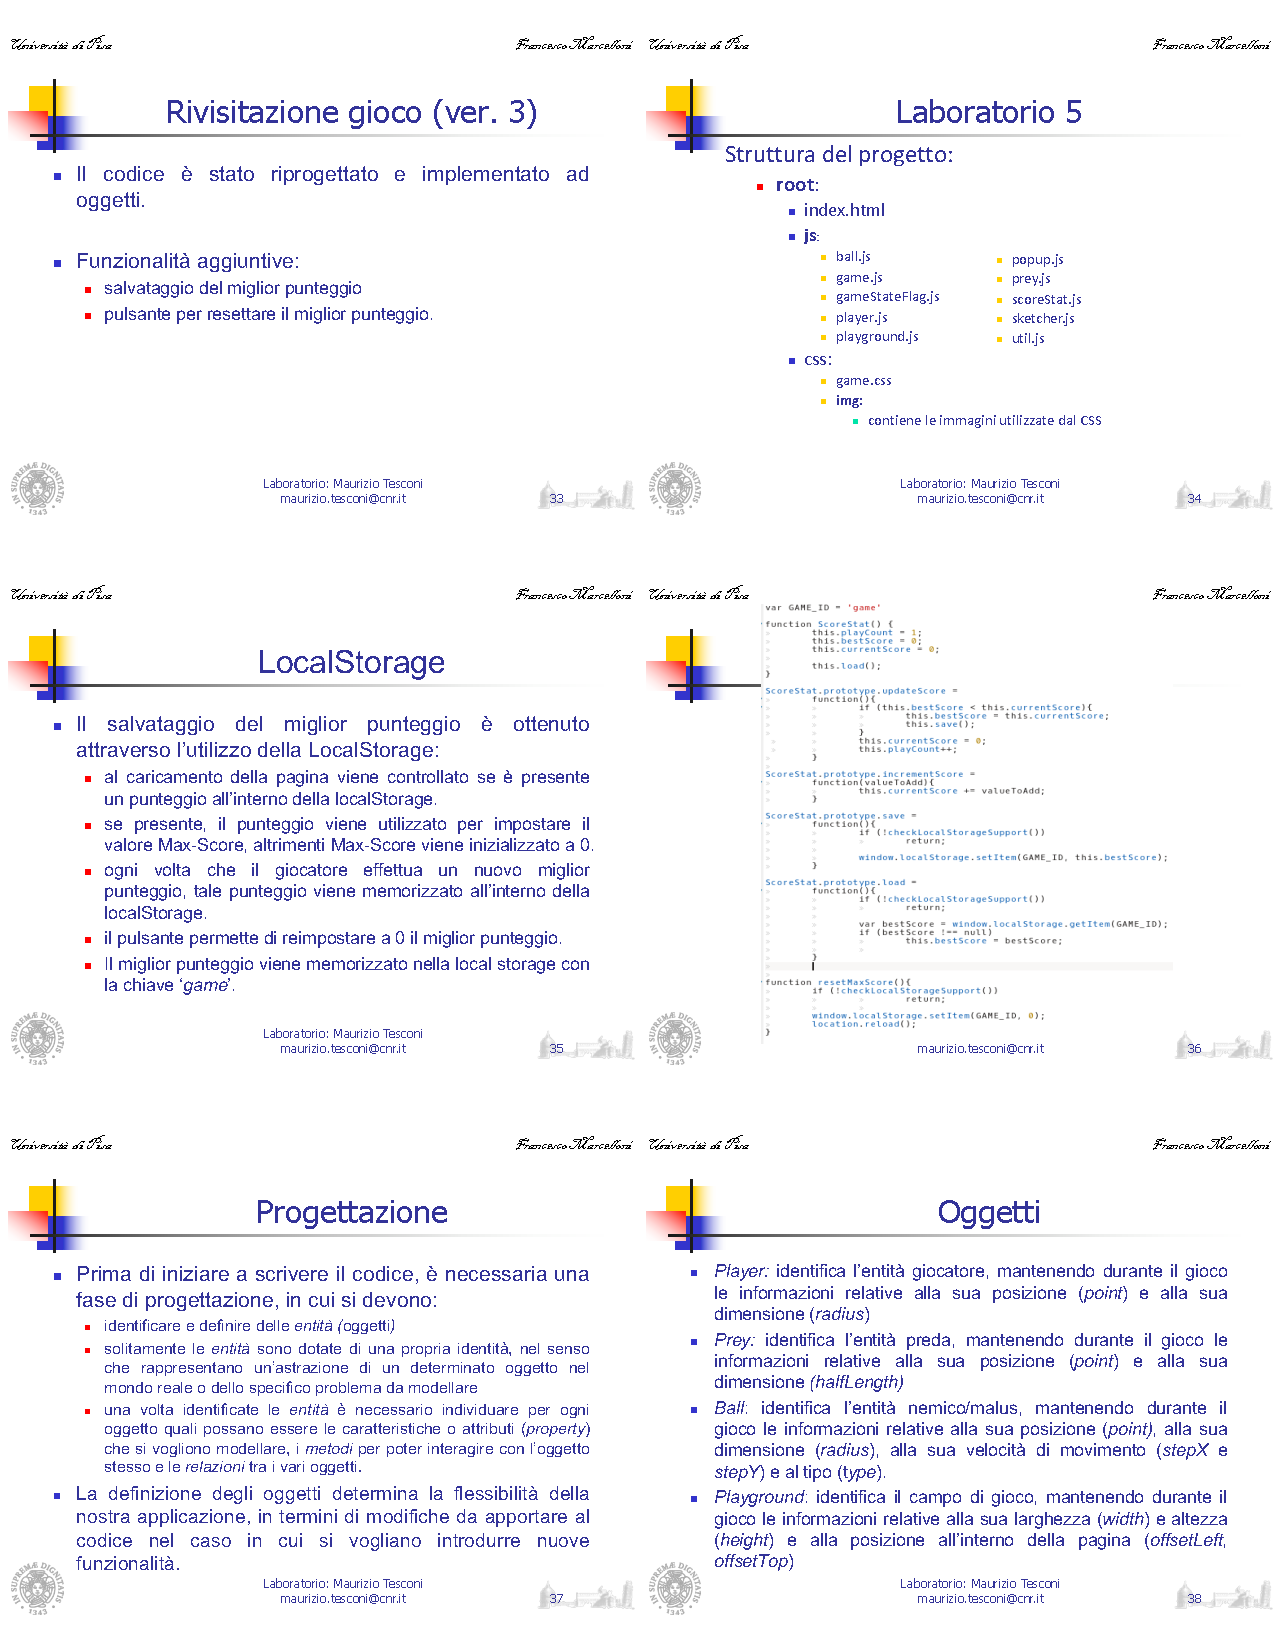
\includepdf[pagecommand={\thispagestyle{plain}},scale=0.88,pages=-]{pdf/iniziolab6}
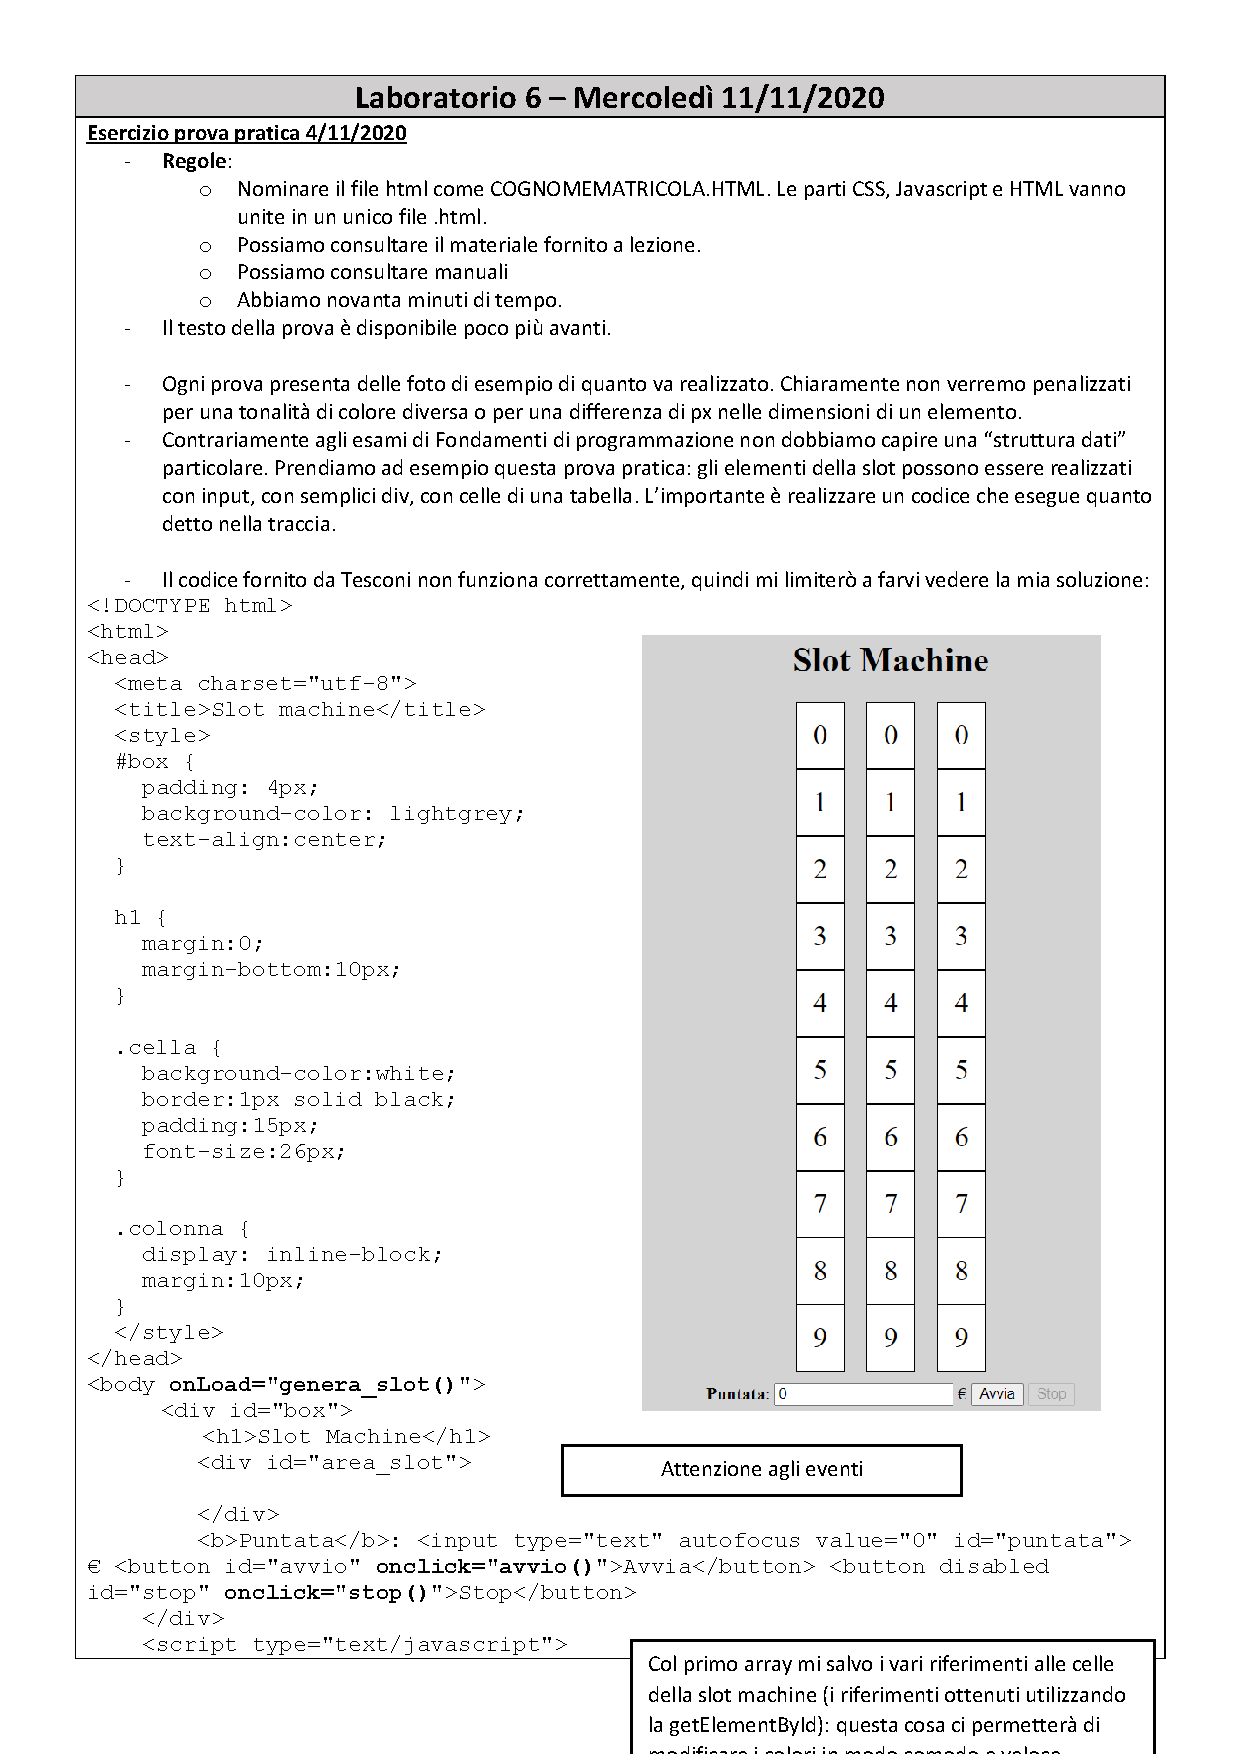
\includepdf[pagecommand={\thispagestyle{plain}},addtotoc={1,chapter,1,{Lab 6 - Mercoledì 11/11/2020},p6},scale=0.92,pages=-]{pdf/lab6}
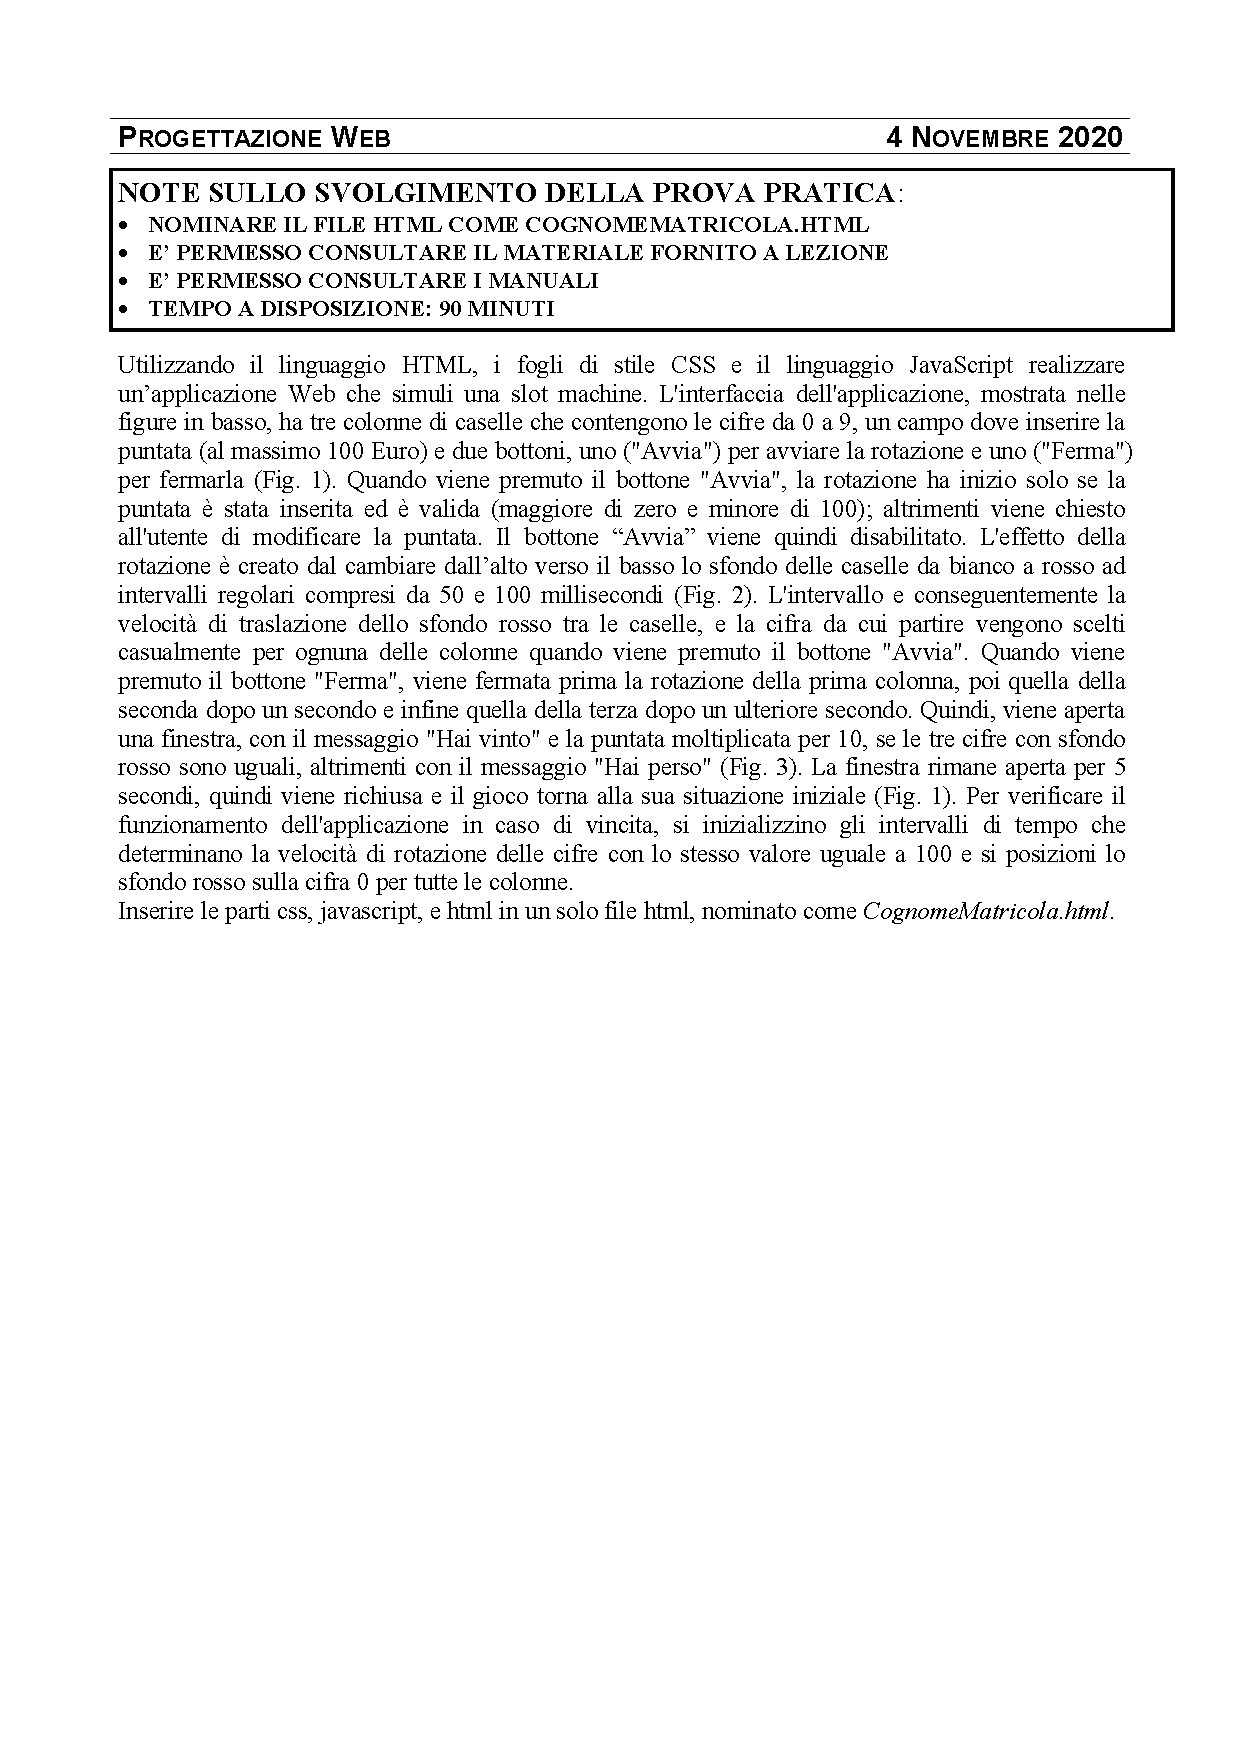
\includepdf[pagecommand={\thispagestyle{plain}},scale=0.95,pages=-]{pdf/esami/compito4Novembre2020}
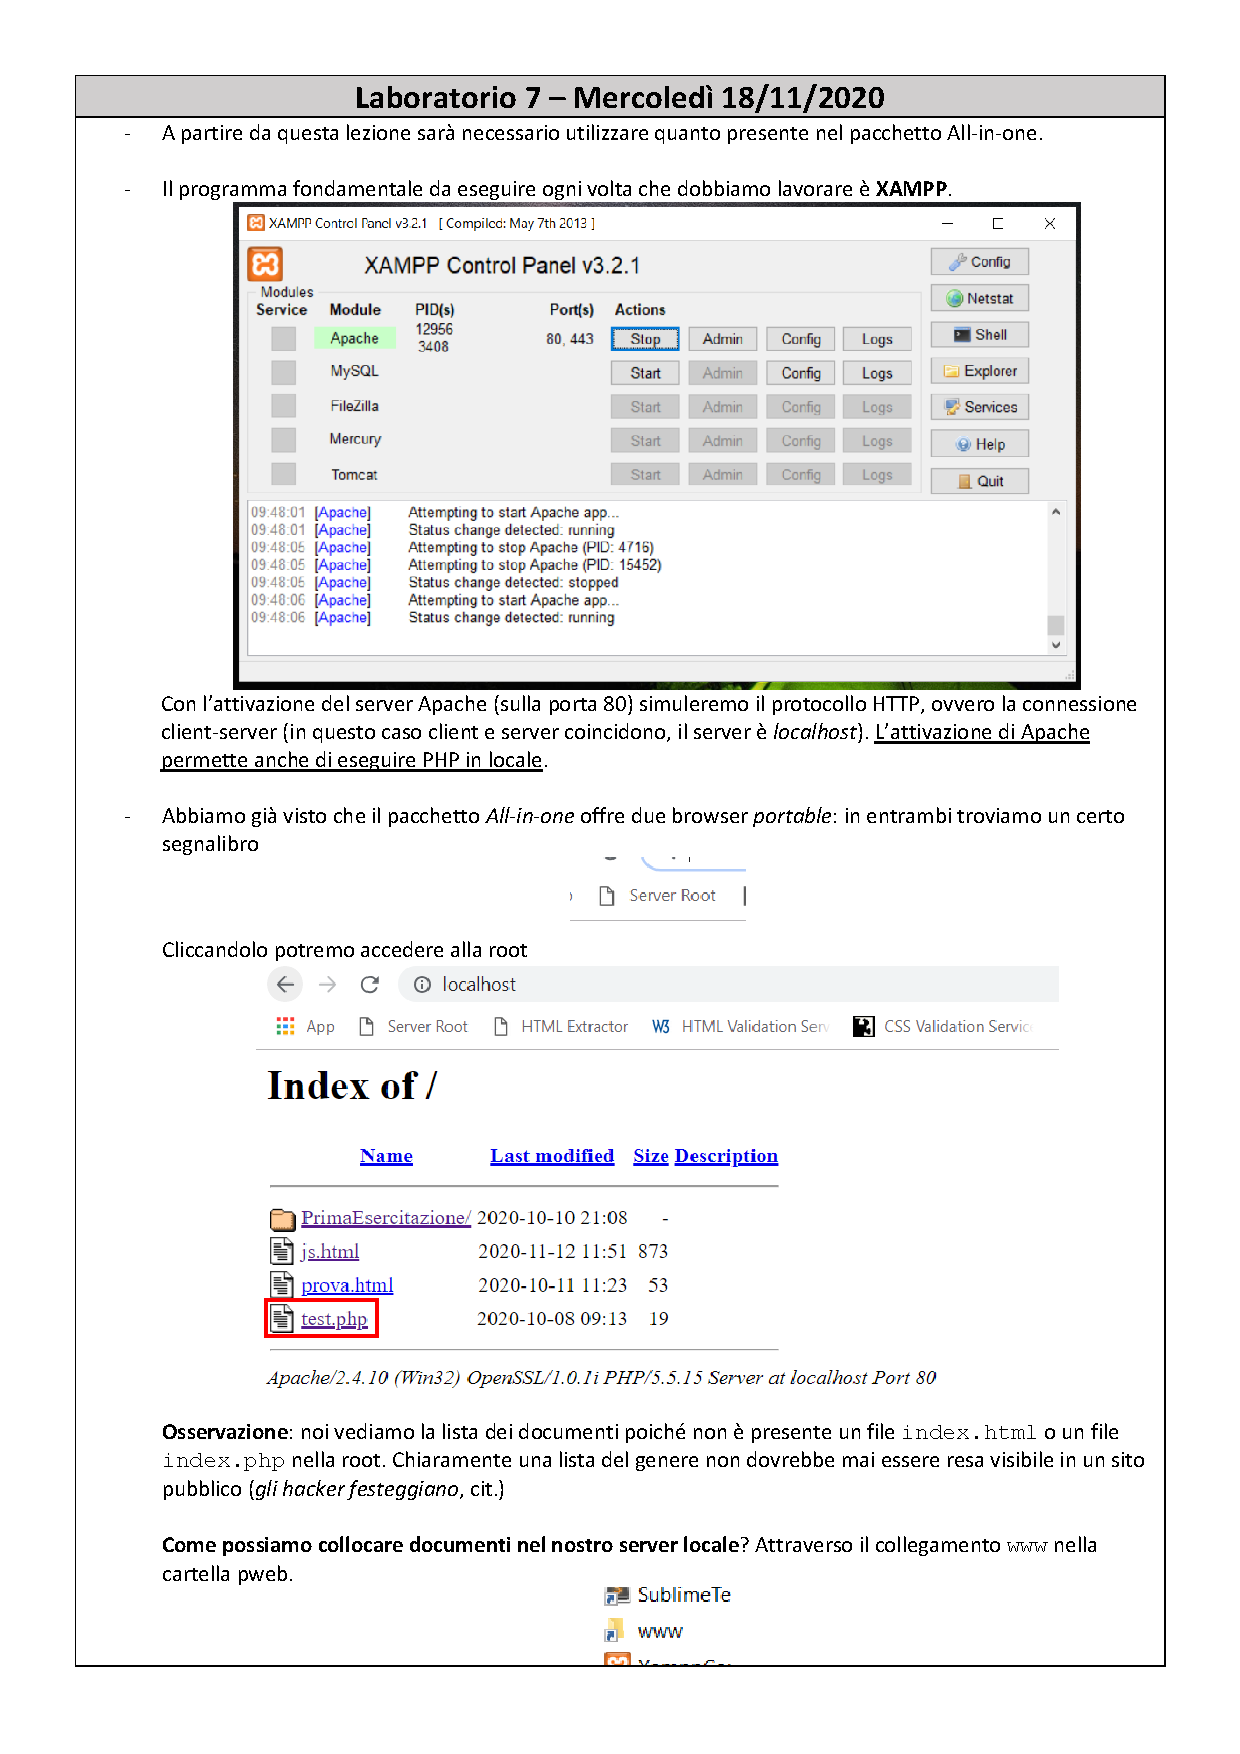
\includepdf[pagecommand={\thispagestyle{plain}},addtotoc={1,chapter,1,{Lab 7 - Mercoledì 18/11/2020},p7},scale=0.92,pages=-]{pdf/lab7}
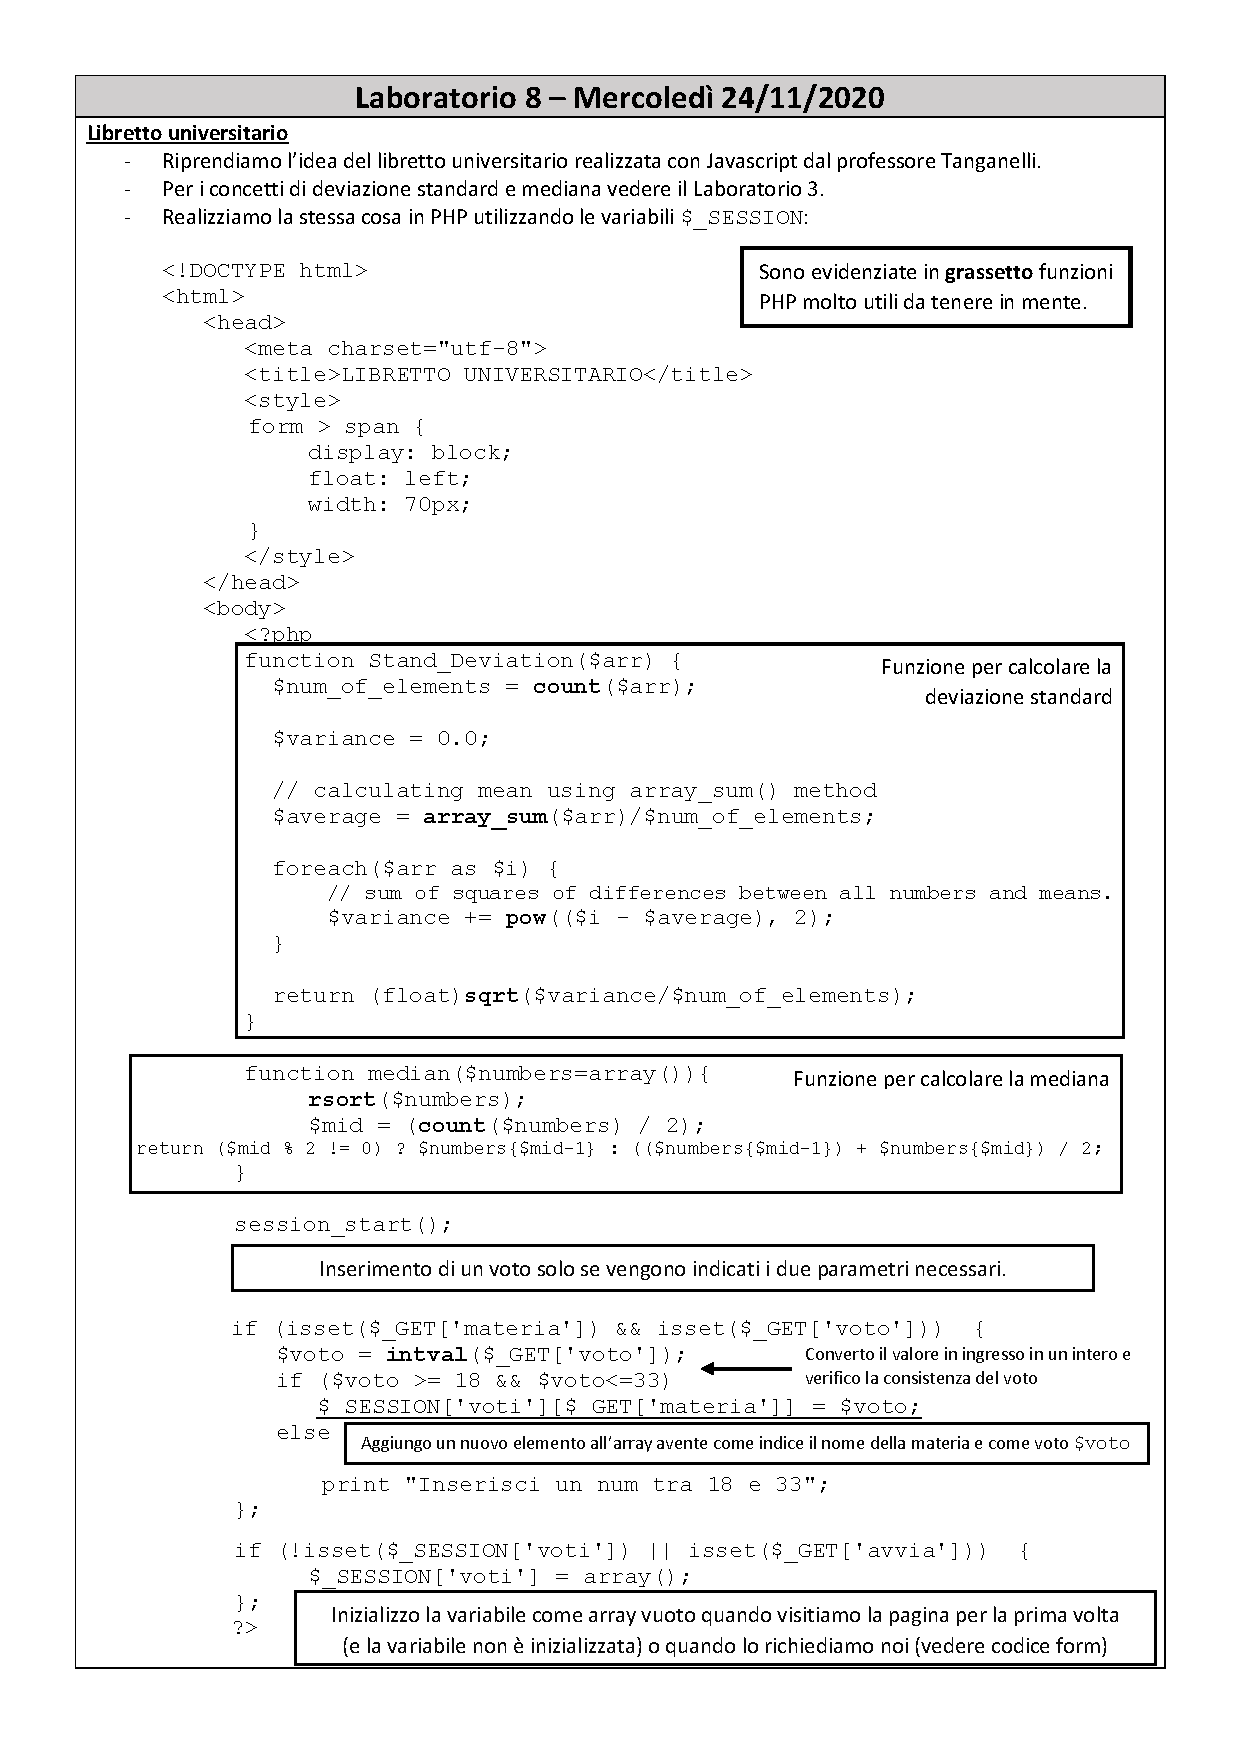
\includepdf[pagecommand={\thispagestyle{plain}},addtotoc={1,chapter,1,{Lab 8 - Mercoledì 24/11/2020},p8},scale=0.92,pages=-]{pdf/lab8}
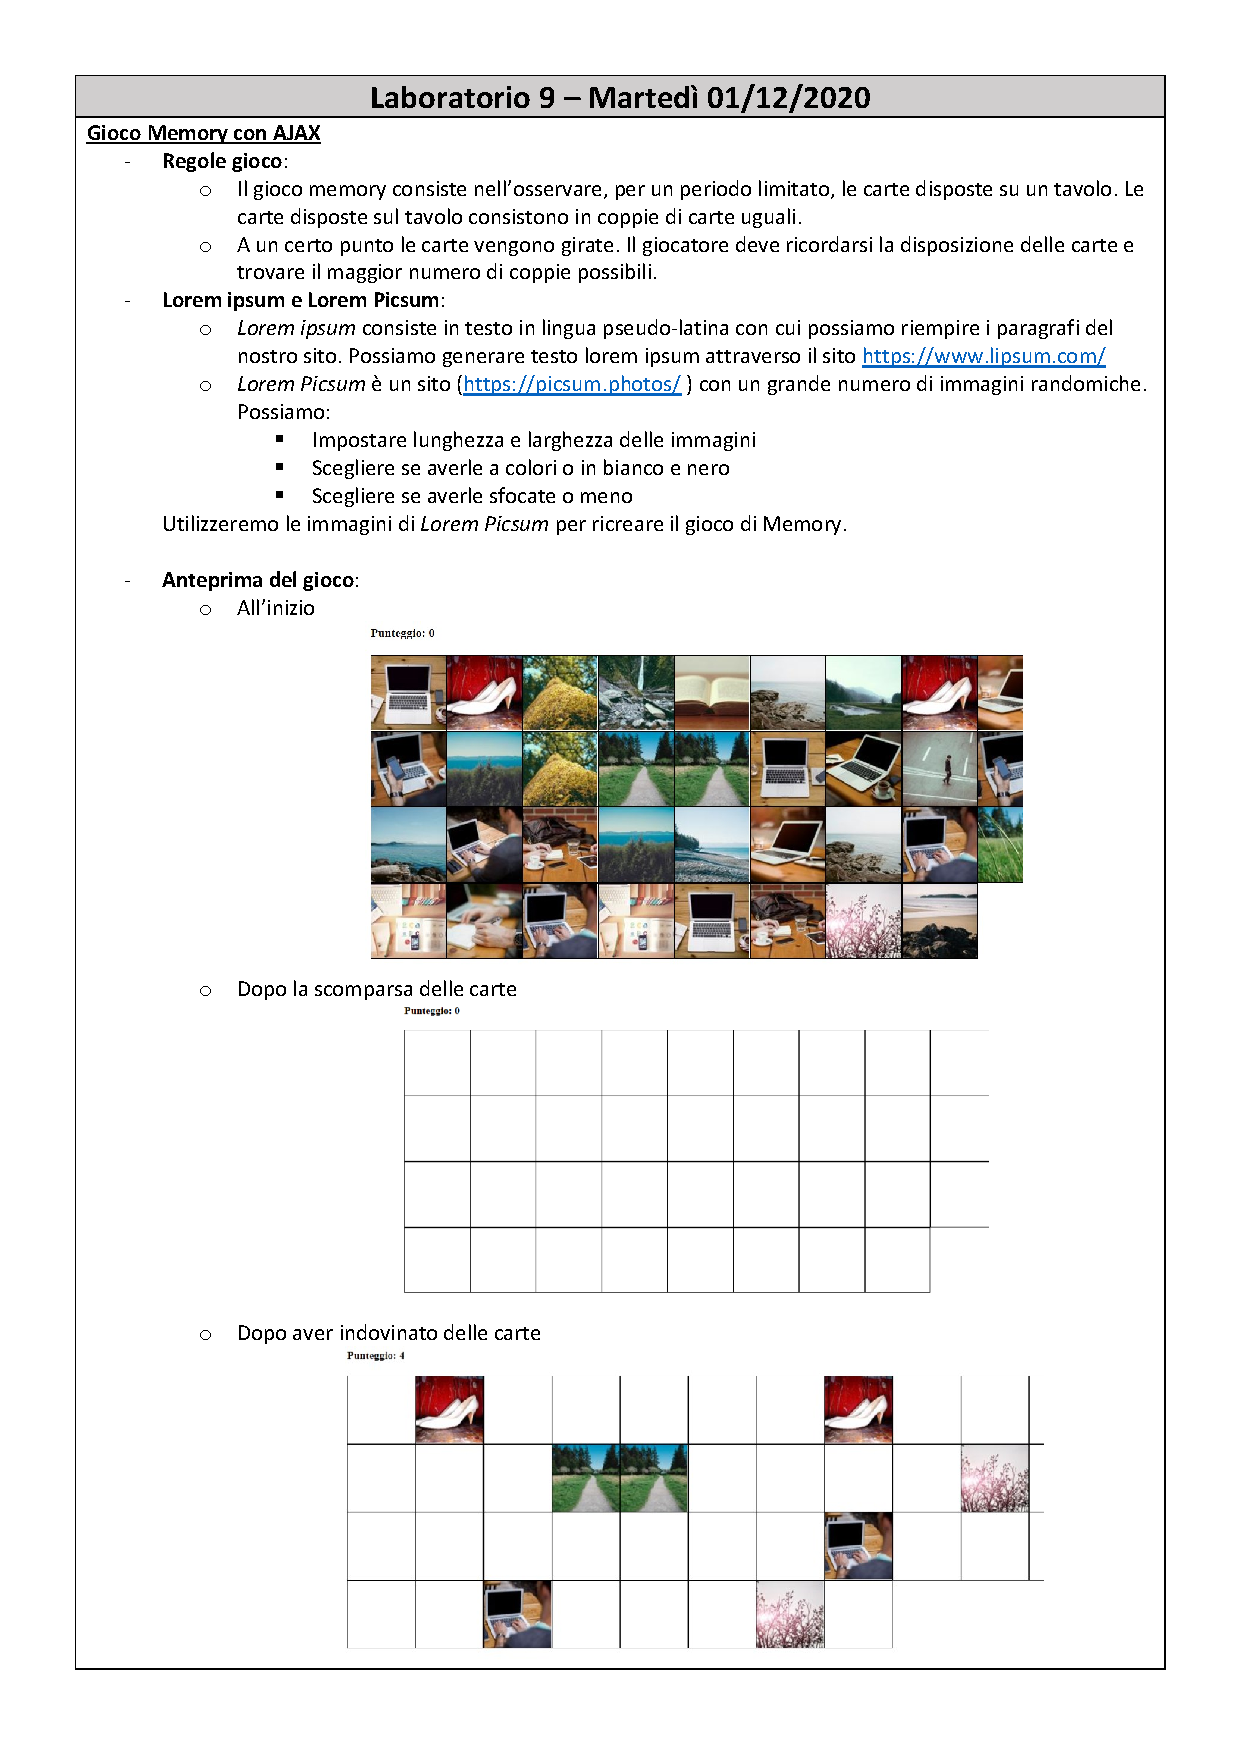
\includepdf[pagecommand={\thispagestyle{plain}},addtotoc={1,chapter,1,{Lab 9 - Martedì 01/12/2020},p9},scale=0.92,pages=-]{pdf/lab9}

 
 
\end{document}
